% ============================================================================
% All frames for the EsT theory deck.  Each frame carries a \note{} that
% becomes the speaker script in est_theory_notes.pdf.
%
% Equation tags cite the PAPER's numbering (arXiv:2603.15356), not the
% numbering in sources/My notes.pdf.  See README.md for the mapping.
% ============================================================================

% ------------------------------------------------------------------ title
\begin{frame}[plain]
  \titlepage
  \note{
    \begin{ntitem}
      \item Paper: Roy, Wetherbee \& Fatemi, arXiv:2603.15356 (7 Apr 2026), Cornell + Berkeley.
      \item Headline claim: a logical gate set $\{X,H,T\}$ on a binomial bosonic qubit that
            stays \emph{almost} error-transparent mid-gate, using only ordinary linear drives.
      \item Result to quote: five-fold reduction in logical infidelity conditioned on a
            photon loss during the gate.
      \item Two halves today. First the paper's theory, up to the three metrics. Then how the
            pulses are found: GRAPE, the model it runs on, the cost function and the
            constraints, with the places our replication differs marked ``ours''. The results,
            simulated and experimental, are a separate talk.
      \item Be explicit that this is the paper's work presented by me, plus our simulation
            replication --- not my result.
      \item Framing sentence to open with: bosonic memories already beat break-even while
            \emph{idling}. This paper is about what breaks when you try to do a \emph{gate}.
    \end{ntitem}}
\end{frame}

% ------------------------------------------------------------------ motivation
\begin{frame}{Why gates are the hard part}
  \begin{itemize}
    \item \textbf{Memories work.} Bosonic codes in a cavity now beat break-even while
          \emph{idling}: the encoded qubit outlives the best uncorrected one.
    \item \textbf{Gates are harder.} A photon lost \emph{during} a gate is pushed around by the
          rest of the gate, and can end up uncorrectable.
    \item \textbf{Error-transparent gates} fix this in principle.
    \item \textbf{This paper:} ordinary linear drives plus \emph{moving} code spaces give $X$,
          $H$, $T$ gates on a binomial code that are \emph{almost} transparent.
  \end{itemize}

  \vfill
  {\color{tagmid}\scriptsize Break-even with bosonic codes: e.g.\ Ni et al., Nature 616 (2023);
  Sivak et al., Nature 616 (2023).}
  \note{
    \begin{ntitem}
      \item One minute, to answer ``why should I care'' before any equations.
      \item Memories: cavity-encoded qubits (binomial, GKP) have been run past break-even ---
            corrected, they live longer than the best uncorrected encoding in the same
            hardware. That is idling only.
      \item Gates: the moment you drive the system, an error that happens mid-gate is
            transformed by the remaining pulse. Unless the gate is designed for it, the error
            that comes out is not the one the code knows how to fix.
      \item Error transparency is the known fix; the paper's abstract notes experiments so far
            have only done phase gates. Their contribution is non-phase gates ($X$, $H$) with
            only standard linear drives, at the price of being only \emph{semi}-transparent.
      \item Quote the headline and attribute it: about five-fold lower infidelity conditioned
            on a photon loss mid-gate, measured. We do not reproduce the experiment.
      \item Then: the first half is the theory of why this is hard and how they measure it; the
            second half is how the pulses are optimised, with our replication marked.
    \end{ntitem}}
\end{frame}

% ------------------------------------------------------------------ roadmap
% Roadmap styles. Defined outside the frame: a frame body is read as a macro
% argument, so a style's #1 inside it breaks.
\tikzset{
  rm idea/.style={draw=#1, line width=0.8pt, rounded corners=3pt, fill=#1!6,
                  text width=2.17cm, minimum height=3.5cm, align=center,
                  inner xsep=4pt, inner ysep=9pt, font=\footnotesize,
                  execute at begin node={\hyphenpenalty=10000\exhyphenpenalty=10000}},
  rm num/.style={circle, fill=#1, text=white, font=\footnotesize\bfseries,
                 inner sep=0pt, minimum size=1.25em},
  rm flow/.style={-{Stealth[length=2.2mm]}, line width=0.9pt, draw=tagmid},
  rm where/.style={font=\scriptsize, text=tagmid, below=3pt},
  rm brace/.style={decorate, decoration={brace, amplitude=5pt}, line width=0.8pt, draw=#1},
}
\begin{frame}{Where we are going}
  \centering
  \begin{tikzpicture}[node distance=0.33cm]
    \node[rm idea=estblue] (b1)
      {\textbf{Correct a loss at rest}\\[5pt] Knill--Laflamme says when; the kitten code qualifies.};
    \node[rm idea=estblue, right=of b1] (b2)
      {\textbf{Keep that through a gate}\\[5pt] Error transparency. With linear drives,
       only \emph{semi}.};
    \node[rm idea=estblue, right=of b2] (b3)
      {\textbf{Measure the shortfall}\\[5pt] Let the code space move: three conditions,
       three metrics.};
    \node[rm idea=codegreen, right=of b3] (b4)
      {\textbf{Optimise the pulse}\\[5pt] GRAPE, on a cost that stands in for the
       conditions.};
    \node[rm idea=codegreen, right=of b4] (b5)
      {\textbf{Check against the paper}\\[5pt] Our $X$ gate next to theirs, and the limits.};

    \foreach \i/\c in {1/estblue, 2/estblue, 3/estblue, 4/codegreen, 5/codegreen}
      \node[rm num=\c] at (b\i.north) {\i};
    \foreach \a/\b in {1/2, 2/3, 3/4, 4/5}
      \draw[rm flow] (b\a.east) -- (b\b.west);

    \node[rm where] at (b1.south) {slides \slideref{device}--\slideref{kittenkl}};
    \node[rm where] at (b2.south) {slides \slideref{gatebreaks}--\slideref{obstruction}};
    \node[rm where] at (b3.south) {slides \slideref{movingcode}--\slideref{metriceta}};
    \node[rm where] at (b4.south) {slides \slideref{grape}--\slideref{constraints}};
    \node[rm where] at (b5.south) {slides \slideref{cmptraces}--\slideref{replication}};

    \draw[rm brace=estblue] ([yshift=11pt]b1.north west) -- ([yshift=11pt]b3.north east)
      node[midway, above=6pt, font=\small\bfseries, text=estblue] {Theory (the paper)};
    \draw[rm brace=codegreen] ([yshift=11pt]b4.north west) -- ([yshift=11pt]b5.north east)
      node[midway, above=6pt, font=\small\bfseries, text=codegreen] {Pulse optimisation};
  \end{tikzpicture}

  \vfill
  {\small Exact transparency is not expected. The paper's move is to make the shortfall
  something we can \emph{measure} (3) and \emph{optimise} (4).}

  \smallskip
  {\color{tagmid}\scriptsize From step 4 on, [ours] marks where our replication differs.}
  \note{
    \begin{ntitem}
      \item Five ideas, one chain. Signpost the argument, not the list of slides.
      \item \textbf{1. Correct a loss at rest.} The device, the Knill--Laflamme condition, and
            the kitten code that meets it. QEC while idling is solved and demonstrated.
      \item \textbf{2. Keep that through a gate.} The natural demand is error transparency:
            a loss during the gate should come out the same as a loss after it. The
            punchline arrives early: with linear drives, exact transparency is not expected,
            only \emph{semi}-transparency.
      \item \textbf{3. Measure the shortfall.} So the paper lets the code and error spaces
            move in time, states three conditions, and gives one number for each.
      \item \textbf{4. Optimise the pulse.} GRAPE finds the drives, with a cost that stands in
            for those conditions and stays inside the hardware limits.
      \item \textbf{5. Check against the paper.} Our simulated $X$ gate against the paper's
            Fig.~1d--f, what agrees and what does not, and what none of this covers.
      \item Emphasise: nothing here makes exact transparency possible. The contribution is
            that the failure becomes \emph{quantifiable and optimisable}.
    \end{ntitem}}
\end{frame}

\section{The system}

% ------------------------------------------------------------------ system Hamiltonian
\begin{frame}{The device: a cavity dispersively coupled to a transmon}
  \slidelabel{device}%
  $\aop$: cavity (storage oscillator, holds the logical qubit).
  $\qop$: transmon (ancilla, for control and parity readout).
  In the dispersive regime:
  \[
    H(t) = H_a + H_q + H_{\mathrm{int}} + H_{\mathrm{drive}}(t)
    \eqin{Eq.~A1}
  \]
  \vspace{-1.8em}
  \begin{align*}
    H_a/\hbar &= \omega_a\,\ad\aop + \tfrac{K}{2}\,\ad{}^{2}\aop^{2}
                 + \tfrac{K'}{6}\,\ad{}^{3}\aop^{3}
                 && \text{\color{tagmid}\scriptsize[A2]}\\
    H_q/\hbar &= \omega_q\,\qd\qop + \tfrac{K_q}{2}\,\qd{}^{2}\qop^{2}
                 && \text{\color{tagmid}\scriptsize[A3]}\\
    H_{\mathrm{int}}/\hbar &= \chi\,\ad\aop\,\qd\qop
                 + \tfrac{\chi'}{2}\,\qd\qop\,\ad{}^{2}\aop^{2}
                 && \text{\color{tagmid}\scriptsize[A4]}\\
    H_{\mathrm{drive}}(t)/\hbar &= \epsilon(t)\,\aop + \Omega(t)\,\qop + \mathrm{h.c.}
                 && \text{\color{tagmid}\scriptsize[A5]}
  \end{align*}

  \vspace{-0.4em}
  {\small
  \begin{tabular}{@{}l r @{\qquad} l r @{\qquad} l r@{}}
    $\chi/2\pi$   & $-3.66$ MHz & $K/2\pi$  & $-22$ kHz  & $K_q/2\pi$ & $-180$ MHz \\
    $\chi'/2\pi$  & $39$ kHz    & $K'/2\pi$ & $590$ Hz   & cavity $T_1$ & $180\ \mu$s
  \end{tabular}}

  \smallskip
  {\color{tagmid}\scriptsize Main-text Eq.~9 is the same Hamiltonian at low order: it drops
  $K'$ and $\chi'$. Values from Table I.}
  \note{
    \begin{ntitem}
      \item Two modes. The cavity $\aop$ is where the logical qubit lives; the transmon $\qop$
            is a nonlinear ancilla we use to steer the cavity and to read out parity.
      \item $H_a$: the cavity's bare frequency, plus self-Kerr $K$ and a smaller
            second-order self-Kerr $K'$. Both make the photon energy depend on how many
            photons are already there.
      \item $H_q$: transmon frequency plus anharmonicity $K_q$. At $-180$~MHz this is what
            makes the transmon usable as a qubit at all --- and it is why the simulation keeps
            three transmon levels, not two.
      \item $H_{\mathrm{int}}$: the dispersive coupling $\chi$, plus a second-order correction
            $\chi'$. Both are photon-number dependent shifts conditioned on the transmon.
      \item $H_{\mathrm{drive}}$: the only thing we control. Two complex amplitudes, linear in
            the mode operators.
      \item These are exactly the numbers and operator forms in \texttt{EST/device.py}.
      \item If asked why the main text shows fewer terms: Eq.~9 is the low-order version;
            App.~A adds $K'$ and $\chi'$, and $\chi'$ matters later --- it is one of the two
            terms that make exact transparency impossible.
    \end{ntitem}}
\end{frame}

% ------------------------------------------------------------------ reading H
\begin{frame}{Reading the Hamiltonian}
  \begin{itemize}
    \item \textbf{Dispersive $\chi$.} $(\omega_q + \chi\,\ad\aop)\,\qd\qop$: the transmon
          frequency moves by $\chi$ per photon, so a transmon drive is
          \emph{photon-number selective}.
    \item \textbf{Kerr $K$, $K'$, $\chi'$.} Small photon-number-dependent shifts. $K$ and
          $\chi'$ (and, weakly, $K'$) are what break error transparency (Eq.~A6).
    \item \textbf{Rotating frame.} Removes $\omega_a$, $\omega_q$; the static part left over
          ($\chi$, Kerr, $K_q$) is the $H_0$ our simulation uses.
    \item \textbf{Controls.} Only the complex $\epsilon(t)$ and $\Omega(t)$, which GRAPE
          shapes.
    \item \textbf{The error the code targets.} Cavity photon loss: jump operator $\aop$,
          rate $\kappa = 1/T_1$.
  \end{itemize}

  \smallskip
  \begin{block}{Notation clash}
    $\epsilon(t)$ is a \emph{drive amplitude}. The noise \emph{channel} on the next slides
    is written $\varepsilon(\rho)$, a different object.
  \end{block}
  \note{
    \begin{ntitem}
      \item The key term is $\chi$. Written as $(\omega_a + \chi\,\qd\qop)\ad\aop$ it is a
            cavity frequency that depends on the transmon; written as
            $(\omega_q + \chi\,\ad\aop)\qd\qop$ it is a transmon frequency that depends on
            photon number. $|\chi|/2\pi = 3.66$~MHz is far larger than the
            transmon linewidth, so the photon-number peaks are resolved: a transmon pulse
            longer than $\sim 1/|\chi|$ ($\approx 270$~ns) can address individual photon
            numbers.
      \item The Kerr-type terms are tiny ($K/2\pi = -22$~kHz), but they do not commute nicely
            with $\aop$. Plant the seed: this is where ``semi'' will come from.
      \item Rotating frame: in the simulation there is no $\omega_a$ or $\omega_q$. What
            remains is the static nonlinearity the pulse has to work with and against.
      \item Photon loss, jump operator $\aop$, is the error the kitten code is designed to
            correct. It is the $E_j$ that will appear in the Kraus form on the next slide.
      \item Flag the symbol clash out loud: drive $\epsilon(t)$ versus channel
            $\varepsilon(\rho)$.
    \end{ntitem}}
\end{frame}

\section{Error correction}

% ------------------------------------------------------------------ setup
\begin{frame}{Setup: code space, projector, errors}
  \slidelabel{setup}%
  A logical qubit lives in a \textbf{code space} $\Cs \subset \mathcal{H}$, with orthonormal
  codewords $\{\ket{c_i}\}$ and projector
  \[
    \PC = \sum_i \proj{c_i} = UU^{\dagger},
    \qquad \PC^{\dagger}=\PC, \quad \PC^{2}=\PC,
  \]
  where $U$ is the encoding isometry ($U^{\dagger}U = \id_{\text{logical}}$).

  \medskip
  Noise is a channel in \textbf{Kraus form}:
  \[
    \varepsilon(\rho) = \sum_j E_j \rho E_j^{\dagger},
    \qquad \sum_j E_j^{\dagger}E_j = \id .
  \]

  \medskip
  \begin{block}{The Kraus set is not unique}
    Any unitary recombination $F_k = \sum_j W_{kj}E_j$ gives the \emph{same} channel.
    We will use this freedom.
  \end{block}
  \note{
    \begin{ntitem}
      \item Two objects, then one warning.
      \item The projector: $P$ is Hermitian and idempotent --- the linear-algebra projection
            onto the code subspace. $U^\dagger U = \id$ on the logical space, but
            $P = UU^\dagger$ is \emph{not} the identity on the full Hilbert space. That
            asymmetry is the whole point of encoding.
      \item The Kraus operators $E_j$ are what we casually call ``the errors''. Same maths as
            simulating decoherence.
      \item The warning is load-bearing, not a footnote: $\{E_j\}$ is only defined up to a
            unitary recombination $W$. The proof of Knill--Laflamme \emph{uses} this to pick
            a basis in which the error matrix is diagonal.
      \item If asked: this is why ``correcting three errors'' and ``correcting a
            three-dimensional span of errors'' are the same statement.
    \end{ntitem}}
\end{frame}

% ------------------------------------------------------------------ KL
\begin{frame}{The Knill--Laflamme theorem}
  \begin{block}{Statement}
    A recovery operation correcting $\{E_a\}$ exists \textbf{if and only if} there is a
    Hermitian matrix $\alpha = (\alpha_{ab})$, $\alpha_{ab}\in\mathbb{C}$, with
    \[
      P_{\Cs}\, E_a^{\dagger} E_b \, P_{\Cs} = \alpha_{ab}\, P_{\Cs}
      \qquad \forall a,b .
    \]
  \end{block}

  \medskip
  Equivalently, in codeword form:
  \[
    \melem{i_L}{E_a^{\dagger}E_b}{j_L} = \alpha_{ab}\,\delta_{ij} .
  \]

  \medskip
  Two independent demands hide in that one equation:
  \begin{itemize}
    \item $\delta_{ij}$: errors must not \textbf{mix} codewords with each other.
    \item $\alpha_{ab}$ \emph{independent of} $i$: the environment must learn nothing
          about \textbf{which} codeword it hit.
  \end{itemize}
  \note{
    \begin{ntitem}
      \item Read the equation aloud in words before unpacking it: sandwich any product of two
            errors between the code projectors, and you must get back the projector itself
            times a number.
      \item ``Proportional to the logical identity'' is the phrase to repeat --- it recurs
            verbatim as Condition 1 later in the talk.
      \item The codeword form makes the two demands visible. Spend time here.
      \item $\delta_{ij}$: no leakage \emph{between} codewords. If $E_a^\dagger E_b$ had an
            off-diagonal piece, an error would rotate $\ket{0_L}$ toward $\ket{1_L}$ and no
            measurement could undo it.
      \item $\alpha_{ab}$ not depending on $i$: no which-path information. This is the
            subtler half and the one the kitten code buys us on the next slides.
      \item Hermiticity of $\alpha$ is automatic --- it comes out of the proof as a Gram
            matrix, hence also positive semidefinite.
      \item Do NOT go through the full proof. The next slide sketches why the condition is
            enough; the derivation is in backup.
    \end{ntitem}}
\end{frame}

% ------------------------------------------------------------------ why KL suffices: sketch
\begin{frame}{Why that condition is enough (sketch)}
  \begin{enumerate}
    \item Diagonalise $\alpha$ and recombine the errors to match (same channel). Then
      \[
        \PC\,F_k^{\dagger}F_l\,\PC = d_k\,\delta_{kl}\,\PC .
      \]
    \item So each error moves the code \textbf{rigidly} onto its own copy $\Cs_k$, and
          different copies are \textbf{orthogonal}.
    \item \textbf{Recovery:} measure which copy (the syndrome), then rotate it back. Outcome $k$
          has probability $d_k$ for every logical state.
  \end{enumerate}

  \vfill
  \plain{errors scatter the code into orthogonal, undistorted copies of itself. Find the copy,
  rotate it back. The measurement learns the error, never the logical state.}

  \smallskip
  {\color{tagmid}\scriptsize Full derivation: backup slides
  B\slideref{klproof}--B\slideref{klrecovery}.}
  \note{
    \begin{ntitem}
      \item This replaces three derivation slides; they are in backup if someone asks.
      \item Step 1 uses the freedom from the setup slide: any unitary recombination of the
            Kraus operators is the same channel. Pick the one that diagonalises $\alpha$.
      \item Step 2: after that, $F_k$ restricted to the code is $\sqrt{d_k}$ times a rigid move
            onto a copy $\Cs_k$, and different $k$ give orthogonal copies.
      \item Step 3: orthogonal copies can be told apart by a projective measurement; rigid
            copies can be rotated back. The outcome probability $d_k$ is the same for every
            code state, so the measurement reveals nothing logical. That is the ``$\alpha$
            independent of $i$'' half of Knill--Laflamme, seen as a measurement property.
      \item Kitten preview: the copies are the even and odd parity sectors, so the syndrome is
            a parity measurement.
    \end{ntitem}}
\end{frame}

\section{The kitten code}

% ------------------------------------------------------------------ kitten code
\begin{frame}{The binomial ``kitten'' code}
  \begin{columns}[T]
    \begin{column}{0.44\textwidth}
      \[
        \ket{0_L} = \frac{\ket{0}+\ket{4}}{\sqrt{2}},
        \qquad
        \ket{1_L} = \ket{2}
      \]
      Both codewords live on the \textbf{even-parity} Fock states.

      \medskip
      A single photon loss $\aop$ sends them to
      \[
        \aop\ket{0_L} = \sqrt{2}\ket{3} \equiv \sqrt{2}\ket{0_E},
      \]
      \[
        \aop\ket{1_L} = \sqrt{2}\ket{1} \equiv \sqrt{2}\ket{1_E},
      \]
      entirely on the \textbf{odd-parity} states. \eqtag{Sec.~III}
    \end{column}
    \begin{column}{0.54\textwidth}
      \centering
      \begin{tikzpicture}[x=0.72cm, y=0.80cm, >=Stealth, font=\scriptsize]
        % even-parity (code) rungs; |2> doubles as |1_L>
        \foreach \n/\lab in {0/{$\ket{0}$}, 2/{$\ket{2}=\ket{1_L}$}, 4/{$\ket{4}$}} {
          \draw[codegreen, line width=1.3pt] (0,\n) -- (1.4,\n);
          \node[anchor=west, inner sep=2pt] at (1.45,\n) {\lab};
        }
        % odd-parity (error) rungs
        \foreach \n in {1,3} {
          \draw[errpurple, line width=1.3pt] (4.5,\n) -- (5.9,\n);
          \node[anchor=west, inner sep=2pt] at (5.95,\n) {$\ket{\n}$};
        }
        % headers
        \node[codegreen, align=center, font=\scriptsize\bfseries] at (1.0,5.5)
             {even parity\\code $\Cs$};
        \node[errpurple, align=center, font=\scriptsize\bfseries] at (5.2,5.5)
             {odd parity\\error $\Es$};
        % |0_L> brackets levels 0 and 4, and the white-filled label breaks the
        % spine exactly at level 2 -- i.e. it visibly skips |1_L>.
        \draw[codegreen, line width=0.8pt] (0,0) -- (-0.55,0) -- (-0.55,4) -- (0,4);
        \node[codegreen, fill=white, inner sep=1.5pt] at (-0.55,2) {$\ket{0_L}$};
        % loss arrows
        \draw[->, line width=0.9pt, black!70] (2.9,4) to[bend left=12] (4.45,3.12);
        \node[anchor=south] at (3.7,3.70) {$\aop$};
        \draw[->, line width=0.9pt, black!70] (3.55,1.95) to[bend left=12] (4.45,1.12);
        \node[anchor=south west, inner sep=1pt] at (3.95,1.55) {$\aop$};
        % a|0> = 0 reminder, below the ladder
        \node[anchor=north, black!55] at (2.6,-0.5) {$\aop\ket{0}=0$};
      \end{tikzpicture}
    \end{column}
  \end{columns}
  \note{
    \begin{ntitem}
      \item One logical qubit in one cavity mode. Two codewords, two error words, five Fock
            levels in total --- hence ``kitten'', a small sibling of the four-legged cat code.
      \item Parity is the organising principle. Codewords are even, loss images are odd, so a
            single parity measurement detects that a loss happened.
      \item Walk the arrows on the diagram. Note $\aop\ket{0}=0$, so only the $\ket{4}$
            component of $\ket{0_L}$ survives the loss: $\aop\ket{0_L}=(0+2\ket{3})/\sqrt2
            = \sqrt2\ket{3}$.
      \item The $\sqrt{2}$ appearing in \emph{both} lines is not a coincidence and it is not
            cosmetic. It is the whole reason this code works --- next slide.
      \item If asked why $\ket{4}$ and not $\ket{6}$: binomial codes are built so the
            codewords' photon-number distributions match to the order of loss you want to
            correct. This one corrects single loss.
    \end{ntitem}}
\end{frame}

% ------------------------------------------------------------------ why correctable
\begin{frame}{Why the kitten code satisfies Knill--Laflamme}
  \slidelabel{kittenkl}%
  Two facts, and they are exactly the two demands from the theorem:
  \begin{enumerate}
    \item \textbf{Distinct, orthogonal images.} $\ket{0_L}\!\to\!\ket{0_E}$,
          $\ket{1_L}\!\to\!\ket{1_E}$ with $\brket{0_E}{1_E} = \brket{3}{1} = 0$.
          Loss acts as an \textbf{isometry} onto the error space, so codewords do not mix.
    \item \textbf{Equal coefficients.} Both images carry the same $\sqrt{2}$, i.e.
          \[
            \melem{0_L}{\ad\aop}{0_L} = \melem{1_L}{\ad\aop}{1_L} = 2 .
          \]
          Equal mean photon number $\Rightarrow$ no which-codeword information.
  \end{enumerate}

  \medskip
  Together:
  \[
    \PC\, \ad\aop\, \PC = 2\,\PC
    \qquad\text{(proportional to the logical identity).}
  \]

  \medskip
  \plain{the environment learns \emph{that} a photon left, and nothing about \emph{which}
  state it left from. No which-path information, so no logical dephasing (to first order
  in $\kappa t$).}
  \note{
    \begin{ntitem}
      \item Map the two facts onto the two halves of Knill--Laflamme explicitly --- this is
            the payoff of having read the equation carefully earlier.
      \item Fact 1 is the $\delta_{ij}$ half. The images are orthogonal, so the loss is an
            isometry onto the error space; logical information is preserved, just relocated.
      \item Fact 2 is the ``$\alpha$ independent of $i$'' half. Both codewords have
            $\bar n = 2$: for $\ket{0_L}$ it is $(0+4)/2 = 2$, for $\ket{1_L}$ it is just 2.
            Photon loss is an amplitude-damping process whose \emph{rate} depends on $\bar n$,
            so matched $\bar n$ means matched loss rate, which means the leak of information
            to the environment carries no logical content.
      \item Say the punchline: the syndrome is the parity flip, even $\to$ odd. Detectable
            and recoverable. This is how bosonic memories beat break-even while idling.
      \item Remember the number 2 --- it comes back as $c_{aa}=2$ in Condition 1.
      \item If asked about dephasing: what would break Fact 2 is the two codewords damping at
            different rates. Then the environment's record correlates with the logical bit and
            you get irreversible logical dephasing, which no end-of-gate recovery can undo.
            App.~A raises exactly this as the reason $\dqec$ is worth minimising.
    \end{ntitem}}
\end{frame}

\section{Error transparency}

% ------------------------------------------------------------------ why gates break QEC
\begin{frame}{Why a gate breaks all of that}
  \slidelabel{gatebreaks}%
  \begin{columns}[c]
    \begin{column}{0.45\textwidth}
      \textbf{Idling.} The codewords barely move (only small Kerr phases). A lost photon
      lands on nearly the same known error word, parity detects it, and you recover.\\[0.8em]
      \textbf{During a gate.} The drive moves the state, so mid-gate it is no longer a
      codeword.
    \end{column}
    \begin{column}{0.53\textwidth}
      \centering
      \begin{tikzpicture}[x=1.00cm, y=0.92cm, >=Stealth, font=\footnotesize]
        % subspace bands
        \fill[codegreen!14, rounded corners=3pt] (1.05,2.30) rectangle (5.70,3.80);
        \fill[errpurple!14, rounded corners=3pt] (1.05,0.15) rectangle (5.70,1.65);
        \node[codegreen, anchor=east, align=right, font=\footnotesize\bfseries]
             at (0.98,3.05) {code\\space};
        \node[errpurple, anchor=east, align=right, font=\footnotesize\bfseries]
             at (0.98,0.90) {error\\space};
        % ideal trajectory, with three tap-off points
        \draw[ordred, line width=1.2pt]
             (1.45,2.80) .. controls (2.70,3.70) and (4.10,2.55) .. (5.35,3.30)
             coordinate[pos=0.00] (s0) coordinate[pos=0.20] (t1)
             coordinate[pos=0.52] (t2) coordinate[pos=0.84] (t3);
        \fill[black] (s0) circle (1.7pt);
        \fill[ordred] (5.35,3.30) circle (1.7pt);
        % losses at three different times land in three different places
        \draw[->, black!65, line width=0.8pt] (t1) -- (1.50,0.60);
        \draw[->, black!65, line width=0.8pt] (t2) -- (3.35,1.15);
        \draw[->, black!65, line width=0.8pt] (t3) -- (5.25,0.45);
        \foreach \pt in {(1.50,0.60), (3.35,1.15), (5.25,0.45)}
          { \fill[errpurple] \pt circle (1.7pt); }
        \node[anchor=south, inner sep=1pt] at (t1) {$t_1$};
        \node[anchor=south, inner sep=1pt] at (t2) {$t_2$};
        \node[anchor=south, inner sep=1pt] at (t3) {$t_3$};
        \node[anchor=west, inner sep=2pt] at (3.42,1.95) {$E_j$};
        \node[errpurple, anchor=north, font=\footnotesize] at (3.40,0.08)
             {three different endpoints};
      \end{tikzpicture}
    \end{column}
  \end{columns}

  \vspace{0.2em}
  \[
    \text{Photon lost at } t\text{:}\quad
    \underbrace{U(T,t)}_{\text{finish}}\;
    \underbrace{E_j}_{\text{loss}}\;
    \underbrace{U(t,0)}_{\text{start}}\ket{\psi_L(0)}
    \quad\text{depends on } t\text{, and } t \text{ is \textbf{random}.}
  \]

  \plain{a photon lost mid-gate ends up somewhere different for every loss time. The
  recovery at the end has one fixed target, so it cannot undo them all.}
  \note{
    \begin{ntitem}
      \item This slide is the hinge of the talk. Do not rush it --- the next equation is
            unmotivated without it.
      \item Idling QEC works because the codewords are nearly \emph{static}. The photon leaves
            while the state sits in the configuration the code was designed around, so the
            loss image is one of two known error words.
      \item Say ``nearly'' on purpose. Kerr is on while idling too, so the error words pick up
            a small phase that depends on when the photon left. Our own check: with no drive at
            all, the trajectory-mismatch metric is already about 0.03. It is the same Kerr effect
            that comes back as the obstruction --- just small when nothing moves.
      \item During a gate that premise is gone. At an intermediate time the state is not a
            codeword at all, just some vector the drive swept it to.
      \item Point at the figure: same ideal trajectory, three loss times, three endpoints.
            The final state is $t$-dependent, and $t$ is a random variable we do not measure.
      \item So end-of-gate recovery has no single target to undo. A syndrome measurement can
            still tell you \emph{that} a photon left, but not how to put the state back.
      \item Set up the next slide as the obvious fix: demand that the jump time stop
            mattering.
    \end{ntitem}}
\end{frame}

% ------------------------------------------------------------------ ET condition
\begin{frame}{Error transparency: the jump commutes through the gate}
  \textbf{The demand:} for all $t\in[0,T]$,
  \[
    U(T,t)\,E_j\,U(t,0)\ket{\psi_L(0)}
      = e^{i\phi_j(t)}\,E_j\,U(T,0)\ket{\psi_L(0)}
      \eqin{Sec.~II}
  \]

  \medskip
  \begin{columns}[T]
    \begin{column}{0.55\textwidth}
      \begin{itemize}
        \item \textbf{Left:} evolve to $t$, get hit by $E_j$, then finish the gate.
        \item \textbf{Right:} finish the whole ideal gate, then get hit, times a
              scalar phase.
      \end{itemize}
      \medskip
      If it holds $\forall t$, a photon lost at \emph{any} time gives the \textbf{ideal gate
      output with one error applied at the end}: a single, known, correctable configuration.
      One recovery at $t=T$ cleans it up.
    \end{column}
    \begin{column}{0.43\textwidth}
      \centering
      \begin{tikzpicture}[x=0.80cm, y=0.82cm, >=Stealth, font=\scriptsize,
                          every node/.style={inner sep=2pt}]
        \node[codegreen] (b)  at (0,2.1) {$\ket{\psi_L(t)}$};
        \node[codegreen] (c)  at (4.0,2.1) {$\ket{\psi_L(T)}$};
        \node[errpurple] (bp) at (0,0) {$E_j\ket{\psi_L(t)}$};
        \node[errpurple] (cp) at (4.0,0) {$E_j\ket{\psi_L(T)}$};
        \draw[->, codegreen, line width=1pt] (b)  -- node[above]{$U(T,t)$} (c);
        \draw[->, errpurple, line width=1pt] (bp) -- node[below]{$U(T,t)$} (cp);
        \draw[->, black!70, line width=1pt]  (b)  -- node[left]{$E_j$} (bp);
        \draw[->, black!70, line width=1pt]  (c)  -- node[right]{$E_j$} (cp);
        \node[estblue] at (2.0,1.05) {$\circlearrowright\; e^{i\phi_j(t)}$};
      \end{tikzpicture}
      \\[0.3em]
      {\color{tagmid}\scriptsize Both routes reach the same state, up to $e^{i\phi_j(t)}$,
      for \emph{every} $t$.}
    \end{column}
  \end{columns}
  \note{
    \begin{ntitem}
      \item State the equation in words first: the two routes around the square agree, up to
            an overall phase that may depend on $t$.
      \item The phase $e^{i\phi_j(t)}$ is free because a global phase is physically
            invisible --- it does not appear in $\rho$.
      \item What this buys: collapse a continuum of possible outcomes (one per jump time)
            into a single outcome. The error becomes \emph{transparent} to the gate --- it
            commutes through, up to a phase.
      \item Concretely: after the gate, you measure parity, find you are in the error space,
            and apply the same recovery you would have used for an idling qubit. The gate
            did not scramble the error.
      \item Heads-up for later: this exact square, with the subspaces allowed to move, is what
            the three conditions in a few slides are designed to enforce.
      \item If asked about multiple losses: the framework is built for single loss, the
            dominant channel for this code. Two-photon events are not covered.
    \end{ntitem}}
\end{frame}

\section{Why only ``semi''}

% ------------------------------------------------------------------ ET as error closure
\begin{frame}{When does a loss commute through? Error closure}
  Push the jump past the Hamiltonian. A loss at any time stays correctable if, at every
  instant, the commutator lands back among the correctable errors:
  \[
    \bigl[\,H(t),\,\aop\,\bigr] \;\in\; \spn\{\text{correctable errors}\}
    \eqin{App.~A}
  \]
  {\color{tagmid}\small This is \emph{error closure}. Exact transparency,
  $[H,\aop] = \lambda\,\aop$, is the special case.}

  \medskip
  Term by term, for the Hamiltonian of slide~\slideref{device}:
  \begin{center}
  \small
  \renewcommand{\arraystretch}{1.3}
  \begin{tabular}{@{}l l l@{}}
    \textbf{Term} & \textbf{Commutator with $\aop$} & \textbf{Correctable?} \\
    \hline
    $\omega_a\,\ad\aop$, \ $\chi\,\ad\aop\,\qd\qop$ & $\propto \aop$ (times $\qd\qop$)
      & {\color{codegreen}yes} \\
    linear drives $\epsilon\,\aop + \Omega\,\qop + \mathrm{h.c.}$ & $-\epsilon^{*}$, a number
      & {\color{codegreen}yes} \\
    Kerr $K$, higher dispersive $\chi'$ & $\propto \ad\aop^{2} = \nop\,\aop$
      & {\color{ordred}no} \\
    \hline
  \end{tabular}
  \end{center}
  \note{
    \begin{ntitem}
      \item Reframe the commuting square as a statement about the Hamiltonian. Moving the jump
            $\aop$ from before $H$ to after it produces the commutator $[H,\aop]$. If that
            commutator is itself a correctable error, a loss at any time still ends as a
            correctable error at $t=T$. That is error closure (App.~A, citing the error-closure
            literature); exact transparency, $[H,\aop] = \lambda\aop$, is the strict special case.
      \item Walk the table. The bare frequencies and the leading dispersive term give $\aop$
            back, times at most a transmon number operator: a deterministic phase on the error
            state (the paper's words).
      \item The linear drives: $[\epsilon\aop + \epsilon^{*}\ad, \aop] = -\epsilon^{*}$, a plain
            number, and the transmon drive commutes with $\aop$. A number times the identity is
            in the correctable set $\{\id, \aop\}$, so linear drives are fine. This is why the
            paper can use the standard cQED toolkit at all.
      \item Then the two that fail: self-Kerr $K$ and the higher-order dispersive $\chi'$. Their
            commutator is $\nop\,\aop$, a jump weighted by photon number --- next slide.
      \item If pressed on the $\chi$ row: the phase depends on the transmon state, and mid-gate
            the transmon is driven. The paper counts it as correctable; the honest statement is
            ``correctable as long as the transmon path is the planned one''.
      \item Why defend linear drives: strong nonlinear drives have been proposed for exact ET,
            but they need strong nonlinearities and tight confinement to the static code space,
            and bring their own spurious processes. The paper's bet is that simpler wins.
    \end{ntitem}}
\end{frame}

% ------------------------------------------------------------------ the obstruction
\begin{frame}{The obstruction: nonlinear terms that will not commute}
  \slidelabel{obstruction}%
  The system Hamiltonian (slide~\slideref{device}) carries the cavity self-Kerr $\tfrac{K}{2}\ad{}^2\aop^2$ and a
  higher-order dispersive term $\tfrac{\chi'}{2}\ad{}^2\aop^2\qd\qop$. Their commutator with
  the jump operator is
  \[
    \left[\;\frac{K}{2}\ad{}^{2}\aop^{2}
           + \frac{\chi'}{2}\ad{}^{2}\aop^{2}\,\qd\qop ,\;\; \aop \;\right]
    = -\bigl(K + \chi'\,\qd\qop\bigr)\,\ad\aop^{2} .
    \eqin{Eq.~A6}
  \]

  \medskip
  \begin{itemize}
    \item $\ad\aop^{2} = \nop\,\aop$ is a jump weighted by photon number. It hits
          $\ket{0_L}$ and $\ket{1_L}$ with different strengths (3 vs 1), so it violates the
          ``$\alpha$ independent of $i$'' half of Knill--Laflamme.
    \item A linear drive can soften its effect along a trajectory, but cannot cancel it: its
          own commutator with $\aop$ is just a number, with no $\nop$-dependent part (App.~A).
  \end{itemize}

  \medskip
  \begin{block}{Therefore: error \emph{semi}transparent}
    Exact ET is not expected with linear drives alone. Accept a small, nonzero violation in
    exchange for simple, standard control, and then \textbf{measure how much you
    recover}.
  \end{block}
  \note{
    \begin{ntitem}
      \item Recall the table on the last slide: the frequencies, the leading $\chi$ and the
            linear drives all pass the error-closure test. Only the nonlinear cavity terms fail.
      \item $K'$ also fails, with a $-\tfrac{K'}{2}\ad{}^2\aop^3$ term. At the photon numbers
            used it is much smaller than the $K$ term (about 40 times at $n=4$), and Eq.~A6
            leaves it out.
      \item The two that break it are the self-Kerr $K$ and the higher-order dispersive
            $\chi'$. Note for yourself: it is $\chi'$, the higher-order coupling, not the
            leading $\chi$ --- and the sign in front of $\chi'$ is PLUS.
      \item Why $\ad\aop^2$ is fatal: write it as $\nop\,\aop$. The $\aop$ is the ordinary
            jump; $\nop$ then weights the result by the photon number left behind. On the
            kitten, $\ket{4}\to\ket{3}$ gets weight 3 and $\ket{2}\to\ket{1}$ gets weight 1.
            Same error space, so the $\delta_{ij}$ demand still holds; but
            $\langle i_L|(\nop\aop)^\dagger\nop\aop|i_L\rangle$ is 18 for $\ket{0_L}$ and 2
            for $\ket{1_L}$, so the error learns which codeword it hit.
      \item Over a gate this shows up as a relative phase of about $2K(T-t)$ between the two
            error words: a logical $Z$ rotation by a random angle, since $t$ is random.
            Averaged over $t$, that is logical dephasing. Roughly 0.28 rad at most for a
            1~$\mu$s gate.
      \item Numbers if asked: $K_a/2\pi = -22$~kHz for the cavity self-Kerr,
            $\chi/2\pi = -3.66$~MHz for the dispersive coupling.
      \item Wording: the paper says exact ET is ``not expected'' here, not that it is proven
            impossible. The commutator shows the operator-level route fails; say that, no more.
      \item Land the word: this is what ``semi'' in error semitransparent names. It is a
            deliberate trade, not a failure to converge. Keep repeating this --- it explains
            why the metrics on trained pulses plateau at a floor.
      \item App.~A's suggested escape routes, if asked: engineer smaller $K$ and $\chi$, keep
            intermediate photon number low, or go to strong nonlinear drives and pay the
            complexity cost.
    \end{ntitem}}
\end{frame}

\section{Instantaneous subspaces}

% ------------------------------------------------------------------ instantaneous code space
\begin{frame}{Letting the code space move}
  \slidelabel{movingcode}%
  The conditions for \emph{static} ET ask the state to stay inside the fixed $\Cs(0)$ and
  $\Es(0)$. Gate drives sweep it far outside both. So: \textbf{track moving subspaces}
  instead.

  \bigskip
  \begin{block}{Instantaneous code space \eqtag{Eq.~1}}
    \vspace{-0.3em}
    \[
      \Cs(t) = \bigl\{\, U(t,0)\ket{\psi_L(0)} \;:\; \ket{\psi_L(0)} \in \Cs(0) \,\bigr\},
      \qquad
      \PC(t) = U(t,0)\,\PC\,U^{\dagger}(t,0) .
    \]
    \vspace{-0.6em}
  \end{block}

  \bigskip
  \begin{itemize}
    \item A 2-dimensional subspace carried along the \textbf{ideal trajectory}.
    \item $U(t,0)$ is the \emph{ideal, lossless} propagator of the driven system.
  \end{itemize}
  \note{
    \begin{ntitem}
      \item This is the paper's central conceptual move, and it is the reason the title says
            ``dynamic encoding subspaces''.
      \item The old framing fails for a trivial reason: a gate has to move the state, so
            insisting it stay inside a fixed two-dimensional subspace rules out the gates we
            want. Earlier exact-ET proposals accepted that and paid for it with strong
            nonlinear drives and very tight confinement.
      \item The fix: define the code space to be wherever the ideal evolution has carried the
            codewords by time $t$. By construction the ideal, lossless trajectory never
            leaves $\Cs(t)$.
      \item Emphasise that this is not a weaker demand in a hand-wavy sense --- it is a
            different, well-posed demand. We still ask for consistency; we just ask for
            consistency with the intended trajectory rather than with a static subspace.
      \item Underline that $U(t,0)$ is the ideal propagator. All three metrics are computed
            from lossless unitary simulation; the loss operator appears only as the algebraic
            object $E_j$, never as an actual quantum jump.
    \end{ntitem}}
\end{frame}

% ------------------------------------------------------------------ instantaneous error space
\begin{frame}{And the error space with it}
  \begin{columns}[T]
    \begin{column}{0.56\textwidth}
      \begin{block}{Instantaneous error space \eqtag{Eq.~2}}
        \[
          \Es_j(t) = \spn\bigl\{\, E_j\ket{\psi_L(t)} \;:\; \ket{\psi_L(t)}\in\Cs(t) \,\bigr\}
        \]
        \[
          \PE{j}(t) \;\propto\; E_j\,\PC(t)\,E_j^{\dagger}
        \]
      \end{block}
      \medskip
      For photon loss, $E_j = \aop$:
      \[
        \Es(t) = \spn\bigl\{\aop U(t,0)\ket{0_L},\; \aop U(t,0)\ket{1_L}\bigr\}
      \]
      \medskip
      \plain{where a photon loss \emph{right now} would send you, given the ideal
      trajectory.}
    \end{column}
    \begin{column}{0.42\textwidth}
      \centering
      \begin{tikzpicture}[x=0.92cm, y=0.80cm, >=Stealth, font=\scriptsize]
        % code tube swept along the ideal trajectory
        \draw[codegreen, line width=0.9pt, fill=codegreen!12]
             (0.2,3.15) .. controls (1.5,4.05) and (2.9,3.05) .. (4.3,3.75) --
             (4.3,3.15) .. controls (2.9,2.45) and (1.5,3.45) .. (0.2,2.55) -- cycle;
        % error tube
        \draw[errpurple, line width=0.9pt, fill=errpurple!12]
             (0.2,1.15) .. controls (1.5,1.75) and (2.9,0.55) .. (4.3,1.35) --
             (4.3,0.75) .. controls (2.9,-0.05) and (1.5,1.15) .. (0.2,0.55) -- cycle;
        \node[codegreen, anchor=south, font=\scriptsize\bfseries] at (2.25,4.10) {$\Cs(t)$};
        \node[errpurple, anchor=north, font=\scriptsize\bfseries] at (2.25,-0.12)
             {$\Es_j(t)$};
        % one time slice
        \draw[black!45, line width=0.7pt, dashed] (2.75,3.62) -- (2.75,0.42);
        \fill[codegreen] (2.75,2.96) circle (1.6pt);
        \fill[errpurple] (2.75,0.86) circle (1.6pt);
        \draw[->, black!70, line width=0.8pt] (2.90,2.85) -- (2.90,1.00);
        \node[anchor=west, inner sep=2pt] at (2.95,1.95) {$\aop$};
        \node[anchor=east, black!60, inner sep=2pt] at (2.68,2.02) {slice at $t$};
        % projectors
        \node[codegreen, anchor=west, font=\scriptsize] at (4.40,3.45) {$\PC(t)$};
        \node[errpurple, anchor=west, font=\scriptsize] at (4.40,1.05) {$\PE{j}(t)$};
      \end{tikzpicture}
    \end{column}
  \end{columns}
  \note{
    \begin{ntitem}
      \item Same move, applied to the error space: push the error space along with the code
            space, so at each instant it is the image of the \emph{current} code space under
            the error.
      \item For this code and this error the error space is again 2-dimensional --- $\aop$
            restricted to the code space has rank 2. Worth flagging: in the repo's own
            implementation this is a real trap; feeding six cardinal states instead of the
            two code words yields four spurious basis vectors outside the error space and
            silently understates leakage.
      \item The proportionality in $\PE{j} \propto E_j\PC E_j^\dagger$ is not an oversight.
            $E_j\PC(t)E_j^\dagger$ is not a projector --- $\aop$ is not unitary, so it does
            not preserve norms. It has to be renormalised, and the paper fixes it only up to
            a constant. At $t=0$ this is exact for the kitten code, because both
            $\aop\ket{0_L}$ and $\aop\ket{1_L}$ have norm $\sqrt 2$ --- the coincidence from
            the Knill--Laflamme slide. Mid-gate that coincidence fails by up to about 20\%.
      \item Point at the figure: two tubes swept along the ideal trajectory. At any time slice
            you have a code 2-space and the error 2-space it maps onto under $\aop$.
      \item Now we have the objects. The next four slides are the conditions that keep the
            commuting square closed on these moving subspaces.
    \end{ntitem}}
\end{frame}

\section{Three conditions}

% ------------------------------------------------------------------ conditions overview
\begin{frame}{The three conditions}
  The dynamic commuting square holds if \textbf{three things are true at every instant}:

  \vfill
  \begin{columns}[T]
    \begin{column}{0.32\textwidth}
      \begin{block}{1. Correctable}
        \centering
        The moving code space is still a valid QEC code.
        \\[0.4em]
        {\color{tagmid}\scriptsize Knill--Laflamme, instant by instant}
      \end{block}
    \end{column}
    \begin{column}{0.32\textwidth}
      \begin{block}{2. Tracking}
        \centering
        The error space goes where the drive carries it.
        \\[0.4em]
        {\color{tagmid}\scriptsize evolved space $=$ instantaneous space}
      \end{block}
    \end{column}
    \begin{column}{0.32\textwidth}
      \begin{block}{3. Matched}
        \centering
        Code and error spaces feel the same internal dynamics.
        \\[0.4em]
        {\color{tagmid}\scriptsize same generator, up to a phase rate}
      \end{block}
    \end{column}
  \end{columns}
  \vfill

  \centering
  {\color{tagmid}\small Each one gets an equation, and later a number that measures how badly
  it is violated.}
  \note{
    \begin{ntitem}
      \item Give the audience the map before the algebra. Three conditions, and later exactly
            one scalar metric per condition --- that pairing is the cleanest way to hold the
            rest of the talk in your head.
      \item One-line intuitions to say out loud:
      \item (1) is a \emph{static} property checked at a moving location --- freeze time, ask
            whether the code you are sitting on could still correct a photon loss.
      \item (2) is about consistency of \emph{history} with \emph{present} --- an error that
            already happened and got carried forward must land in the same place as an error
            happening now.
      \item (3) is about \emph{rates} --- even if the two subspaces coincide, the drive must
            not rotate the state differently inside them.
      \item Note that (2) and (3) are genuinely independent: (2) is about which subspace you
            are in, (3) is about where inside it you are.
    \end{ntitem}}
\end{frame}

% ------------------------------------------------------------------ condition 1
\begin{frame}{Condition 1: instantaneous correctability}
  Over the error set $E = \{\id,\ \aop\}$, every projected error product must be
  \textbf{proportional to the logical identity}:
  \[
    \PC(t)\, E_i^{\dagger} E_j \,\PC(t) = c_{ij}(t)\, \PC(t),
    \qquad \forall i,j,t .
    \eqin{Eq.~3}
  \]
  This is Knill--Laflamme again, now demanded of the code space \emph{as it moves}.

  \vspace{1.4em}
  \begin{columns}[T]
    \begin{column}{0.46\textwidth}
      \textbf{The kitten code at $t=0$:}
      \[
        c(0) =
        \begin{pmatrix} c_{II} & c_{Ia} \\ c_{aI} & c_{aa} \end{pmatrix}
        = \begin{pmatrix} 1 & 0 \\ 0 & 2 \end{pmatrix}
      \]
    \end{column}
    \begin{column}{0.52\textwidth}
      At $t=0$ the only live entry is $c_{aa}$, and $\ad\aop=\nop$, so it is the demand
      \[
        \melem{0_L}{\nop}{0_L} = \melem{1_L}{\nop}{1_L} \;(=2).
      \]
    \end{column}
  \end{columns}

  \note{
    \begin{ntitem}
      \item Point out that this is literally the Knill--Laflamme equation from earlier, with
            $\PC \to \PC(t)$. Nothing new mathematically; the content is the $t$.
      \item The error set is $\{\id, \aop\}$ --- identity plus single photon loss --- so there
            are four ordered pairs and hence four $2\times2$ blocks.
      \item Walk the matrix. $c_{II}=1$: trivial, the code words stay orthonormal under
            unitary evolution, so that block is exactly the identity and contributes nothing.
            Off-diagonals vanish: $\melem{0_L}{\aop}{1_L}=0$ because $\aop\ket{2}
            \propto \ket{1}$ which is orthogonal to both code words, and likewise the other
            way. So the only live entry is $c_{aa}$.
      \item $c_{aa} = 2$ is the number from the kitten-code slide: $\bar n = 2$ for both code
            words. Call back to it explicitly --- the audience saw it twenty minutes ago.
      \item Do not oversell the $t=0$ picture. Matched $\bar n$ is only one component of one
            block. Mid-gate the drive mixes parities, so $\melem{0_L(t)}{\aop}{1_L(t)}$ and the
            off-diagonal parts of the $(\aop,\aop)$ block need not vanish. Matched $\bar n$ is
            necessary, not sufficient.
      \item Why it can fail: photon loss is amplitude damping, and its rate scales with
            $\bar n$. If the drive pushes $\ket{0_L}$ to a higher $\bar n$ than $\ket{1_L}$,
            they damp at different rates, the environment's record correlates with the
            logical bit, and you get logical dephasing --- irreversible, and not something the
            standard end-of-gate recovery can undo. App.~A makes exactly this point.
      \item Presentational note to self: the paper's Eq.~A7 defines an optional penalty
            $\Delta\bar n_L(t)$ that enforces just this. It is available but not part of the
            default objective --- that comes up again on the cost-function overview.
    \end{ntitem}}
\end{frame}

% ------------------------------------------------------------------ condition 2
\begin{frame}{Condition 2: subspace tracking}
  \[
    U(t,0)\,\Es_j(0) = \Es_j(t), \qquad \forall j,t .
    \eqin{Eq.~4}
  \]

  Two different objects that must coincide:
  \begin{itemize}
    \item \textbf{Evolved} $U(t,0)\Es_j(0)$: where a jump at $t=0$ has been
          \emph{carried to} by now.
    \item \textbf{Instantaneous} $\Es_j(t)$: where a jump \emph{right now} would land.
  \end{itemize}

  \begin{block}{Why anchoring at $t=0$ is enough}
    A jump can happen at any time $s$. Right after it the state is in $\Es_j(s)$, and the
    drive carries it to $U(T,s)\,\Es_j(s)$ by the end $T$.
    \[
      U(T,s)\,\Es_j(s)
      \underset{\text{Eq.~4 at } s}{=} U(T,s)\,U(s,0)\,\Es_j(0)
      \underset{\text{compose}}{=} U(T,0)\,\Es_j(0)
      \underset{\text{Eq.~4 at } T}{=} \Es_j(T).
    \]
    So an error $j$ always ends in the same subspace $\Es_j(T)$, whenever it happened.
  \end{block}
  \note{
    \begin{ntitem}
      \item The equation is short; the content is in distinguishing the two objects. Spend the
            time there and use the tube picture from two slides ago.
      \item ``Evolved'' is a statement about history: the jump happened at $t=0$ and the drive
            has been pushing the resulting state around ever since.
      \item ``Instantaneous'' is a statement about the present: if the jump happened right
            now, from the current code space, where would it put you?
      \item Condition 2 says these are the same subspace. If they are not, then whether a
            recovery works depends on when the jump happened --- which is exactly the
            $t$-dependence we set out to eliminate.
      \item Anticipate the obvious objection, because someone will raise it: the equation only
            ever compares time $t$ against time $0$, but jumps happen at all times.
      \item Walk the block left to right. Eq.~4 at time $s$ rewrites the space the jump lands
            in as an evolved copy of $\Es_j(0)$. The two propagators then merge into one,
            $U(T,s)U(s,0) = U(T,0)$. Eq.~4 at time $T$ turns that back into $\Es_j(T)$.
      \item The punchline is that $s$ drops out. Where the state ends up does not depend on
            when the jump happened, so the final recovery does not need to know it. $t=0$
            is a sufficient anchor because the propagator composes.
      \item Connect forward: this is the condition that the leakage metric $\Lleak$ measures.
    \end{ntitem}}
\end{frame}

% ------------------------------------------------------------------ condition 3
\begin{frame}{Condition 3: matched internal dynamics}
  With $P_j(t) \propto E_j\PC(t)$ the map carrying the code space onto the instantaneous
  error space (an isometry up to normalisation),
  \[
    P_j^{\dagger}(t)\,H(t)\,P_j(t)
    = \PC^{\dagger}(t)\,H(t)\,\PC(t) + d_j(t)\,\PC(t),
    \qquad \forall j,t ,
    \eqin{Eq.~5}
  \]
  where $d_j(t)$ is a number. The paper calls it complex; both sides are Hermitian, so it is
  real.

  \medskip
  Read as Hamiltonians restricted to the two subspaces:
  \[
    H_{\Es}(t) = H_{\Cs}(t) + d_j(t)\,\id .
  \]

  \medskip
  \begin{itemize}
    \item The two subspaces are driven by the \textbf{same generator}, differing only by a
          multiple of the identity.
    \item A shift proportional to $\id$ is a global phase rate, physically invisible.
  \end{itemize}

  \medskip
  \centering
  \plain{the drive must push the error space around in exactly the same way it pushes the
  code space, apart from an overall phase.}
  \note{
    \begin{ntitem}
      \item Conditions 1 and 2 are about \emph{which subspace} you occupy. Condition 3 is
            about \emph{where inside it} you are. That distinction is the reason all three are
            needed.
      \item Even if the error space tracks perfectly, the drive could rotate the state within
            the error space differently from how it rotates the code state. Then the logical
            content of the two would drift apart, and the error would no longer commute
            through the gate.
      \item $P_j$ is not a projector: it maps one space to another, like the undistorted-copy
            maps in the Knill--Laflamme sketch. So $P_j^{\dagger}HP_j$ is the error-space Hamiltonian pulled back onto the
            code space, which is what lets the two sides be compared.
      \item $d_j$ is real: both sides of Eq.~5 are Hermitian, so their difference is too. An
            imaginary part would change the norm of the state, not just its phase.
      \item $d_j(t)\id$ is the allowed slack, and it is exactly the right amount of slack: a
            term proportional to the identity generates a global phase, which is invisible in
            $\rho$. Tie this back to $e^{i\phi_j(t)}$ on the commuting-square slide --- it is
            the same freedom, expressed at the level of the generator instead of the state.
      \item Anything beyond that --- any relative rotation --- is a real, physical mismatch.
            That is what the trajectory-mismatch metric $\etam$ will measure.
      \item If asked how this connects to the App.~A obstruction: the uncorrectable
            $\ad\aop^2$ commutator is precisely a term that fails Condition 3, because it
            generates a photon-number-dependent \emph{relative} rotation, not a multiple of
            the identity.
    \end{ntitem}}
\end{frame}

\section{Three metrics}

% ------------------------------------------------------------------ metrics overview
\begin{frame}{Three metrics, one per condition}
  Each condition gets a scalar that is \textbf{zero when the condition holds}.

  \vfill
  \begin{center}
  \small
  \renewcommand{\arraystretch}{1.5}
  \begin{tabular}{@{}c l l@{}}
    \textbf{Condition} & \textbf{Metric} & \textbf{Question it answers} \\[0.2em]
    \hline
    1 & QEC violation $\dqec(t)$ \eqn{Eq.~6}
      & Is the moving code still correctable? \\
    2 & Leakage $\Lleak(t)$ \eqn{Eq.~7}
      & Is the error state in the right subspace? \\
    3 & Trajectory mismatch $\etam(t)$ \eqn{Eq.~8}
      & Is it in the right place inside it? \\
    \hline
  \end{tabular}
  \end{center}
  \vfill

  All three are \textbf{time-dependent}: they are evaluated at every step of the pulse, not
  just at $t=T$.
  \note{
    \begin{ntitem}
      \item The pairing is the thing to sell here. Three conditions, three numbers, one-to-one.
      \item All three are computed from \emph{lossless} unitary simulation. No quantum jumps
            are simulated; $E_j$ enters only as an algebraic object. That is worth saying
            explicitly because it surprises people --- these are properties of the ideal
            evolution, not of a stochastic trajectory.
      \item Time dependence matters: a pulse can look perfect at $t=T$ and be badly
            non-transparent in the middle, and the middle is exactly where a random photon
            loss might strike. This is why the cost function has to sum over the whole
            trajectory rather than just score the endpoint.
      \item Flag now, expand in the cost-function section: these are \emph{diagnostics}. The
            optimiser's actual cost function is a different, differentiable object built from
            state overlaps.
    \end{ntitem}}
\end{frame}

% ------------------------------------------------------------------ metric 1
\begin{frame}{Metric 1: QEC violation $\dqec(t)$}
  Form the $2\times2$ projected error matrices, over $E=\{\id,\aop\}$:
  \[
    M_{ik}(t) = \PC(t)\,E_i^{\dagger}E_k\,\PC(t)
    = c_{ik}\PC + x_{ik}X_{\Cs} + y_{ik}Y_{\Cs} + z_{ik}Z_{\Cs} .
    \eqin{Eqs.~A8--A9}
  \]
  The $\PC$ part is correctable; the $X,Y,Z$ parts are \textbf{not}. So strip the identity
  and measure what is left:
  \[
    \dqec(t) = \sum_{i,k}
      \Bigl\| M_{ik} - \tfrac{1}{2}\Tr\!\left[M_{ik}\right]\PC \Bigr\|_2
    = \sum_{i,k} 2\bigl(|x_{ik}|^2 + |y_{ik}|^2 + |z_{ik}|^2\bigr) .
    \eqin{Eqs.~6, A11}
  \]

  \medskip
  \centering
  \plain{$\dqec(t) = 0$ means a photon lost at time $t$ can still be corrected. Larger means a
  bigger uncorrectable part. It is a size, not a probability.}

  \medskip
  {\color{tagmid}\scriptsize $\|A\|_2 = \Tr(A^{\dagger}A)$ is the squared Frobenius norm
  (App.~A): no square root, hence the factor of 2.}
  \note{
    \begin{ntitem}
      \item Structure the explanation as three moves: build the matrix, expand it, throw away
            the harmless part.
      \item Build: $M_{ik}$ is Condition 1's left-hand side. Condition 1 wanted every
            $M_{ik}$ proportional to $\PC$; this metric measures the failure of exactly that.
      \item Expand: $\PC(t)$ acts as the identity inside the 2-dimensional logical space, so
            $\{\PC, X_\Cs, Y_\Cs, Z_\Cs\}$ is a complete basis and the expansion is unique.
      \item Strip: $\Tr[M_{ik}] = 2c_{ik}$ because the logical Paulis are traceless and
            $\Tr\PC = 2$. So subtracting $\tfrac12\Tr[M_{ik}]\PC$ removes precisely the
            correctable piece, leaving only uncorrectable generators.
      \item Note to self on the norm --- this is the one place my own notes are wrong. I wrote
            $\|A\|_2 = \sqrt{\lambda_{\max}(A^\dagger A)}$, the spectral norm, but then quoted
            the answer $2(|x|^2+|y|^2+|z|^2)$, which is the Frobenius result. The main text
            says ``2-norm'' but sends you to App.~A, and App.~A defines
            $\|A\|_2 = \Tr(A^\dagger A)$ with no square root. Frobenius is the right reading,
            and it is what our own implementation uses.
      \item The $(\id,\id)$ pair contributes exactly zero: $M_{II} = \PC$ is pure
            identity, because unitary evolution keeps the code words orthonormal.
      \item Not normalised by anything --- so absolute values are directly comparable to the
            paper's.
    \end{ntitem}}
\end{frame}

% ------------------------------------------------------------------ metric 2
\begin{frame}{Metric 2: instantaneous leakage $\Lleak(t)$}
  \[
    \Lleak(t) = 1 - \Tr\bigl[\, \PE{j}(t)\,\rho(t) \,\bigr]
    \eqin{Eq.~7}
  \]
  where $\rho(0)$ is the \textbf{maximally mixed state in the static error space}
  $\Es_j(0)$, evolved unitarily with no losses:
  \[
    \rho(0) = \frac{\PE{j}(0)}{d} = \tfrac{1}{2}\bigl(\proj{0_E} + \proj{1_E}\bigr),
    \qquad
    \rho(t) = U(t,0)\,\rho(0)\,U^{\dagger}(t,0) .
  \]

  \medskip
  So the trace compares two subspaces: the \textbf{evolved} error space (carried in $\rho(t)$)
  against the \textbf{instantaneous} one (in $\PE{j}(t)$). That is exactly Condition 2.

  \medskip
  \centering
  \plain{the probability, averaged over all logical inputs, that a state which suffered
  the error at $t=0$ is found \emph{outside} the subspace an error at time $t$ would
  produce.}
  \note{
    \begin{ntitem}
      \item Unpack why the maximally mixed state is the right initial condition: it is
            proportional to the projector, so $\Tr[\PE{j}(t)\rho(t)]$ is an average over all
            logical inputs rather than a statement about one particular state. That is what
            makes this a property of the \emph{subspace} and not of a chosen vector.
      \item For the kitten code, $\PE{j}(0) = \proj{1} + \proj{3}$, so
            $\rho(0) = \tfrac12(\proj{1}+\proj{3})$.
      \item The key identity that makes this a subspace-overlap: for any state,
            $\Tr[P\proj{\phi}] = \melem{\phi}{P}{\phi}$. So the trace expands into the mean
            of $\melem{0_E(t)}{\PE{j}(t)}{0_E(t)}$ and the same for $\ket{1_E(t)}$ --- the
            alignment of the two error subspaces.
      \item Emphasise the evolved-versus-instantaneous framing; it is the same distinction as
            Condition 2 and this is its scalar.
      \item Worth stating: no loss is ever applied during the evolution. The error is applied
            once, at $t=0$, and then everything is unitary.
      \item If asked how this differs from $\etam$: leakage asks whether you are in the right
            \emph{subspace}; $\etam$ asks, given that you are, whether you are at the right
            \emph{place inside it}. $\etam$ projects the error state into the instantaneous
            error space first, which makes it deliberately blind to leakage. So the two carry
            genuinely independent information, and neither bounds the other.
    \end{ntitem}}
\end{frame}

% ------------------------------------------------------------------ metric 3
\begin{frame}{Metric 3: trajectory mismatch $\etam(t)$}
  \slidelabel{metriceta}%
  \[
    \etam(t) = \bigl\| \vec r_{\Cs}(t) - \vec r_{\Es_j}(t) \bigr\|_2 \;\in [0,2]
    \eqin{Eq.~8}
  \]
  \[
    \vec r_{\Cs}(t) = \Tr\bigl[\vec\sigma_{\Cs}(t)\,\rho_{\ket{\psi}}(t)\bigr],
    \qquad
    \vec r_{\Es_j}(t) = \Tr\bigl[\vec\sigma_{\Es_j}(t)\,\tilde\rho_{\ket{\psi_{E_j}}}(t)\bigr]
  \]

  \medskip
  \begin{itemize}
    \item Take a logical state $\ket{\psi}$ and its error partner
          $\ket{\psi_{E_j}} \propto E_j\ket{\psi}$; evolve both.
    \item Write each as a Bloch vector in \textbf{its own} instantaneous logical frame
          ($\vec\sigma_{\Cs}(t)$ in the code space, $\vec\sigma_{\Es_j} \propto
          E_j\vec\sigma_{\Cs}E_j^{\dagger}$ in the error space), and measure the distance.
    \item The error state is \emph{projected into} $\Es_j(t)$ first, so $\etam$ is blind to
          leakage: independent information from $\Lleak$.
    \item Evaluated over all 6 Bloch cardinal states.
  \end{itemize}

  \medskip
  \centering
  \plain{``where is the state on the code sphere?'' vs.\ ``where is it on the error
  sphere?'' Zero means no relative rotation (Condition 3).}
  \note{
    \begin{ntitem}
      \item The picture to describe: two Bloch spheres side by side, one for the code space
            and one for the error space, each carried along by the drive. Put a state on the
            code sphere and its error partner on the error sphere. At $t=0$ they sit at the
            same point. Transparency says they must stay at the same point.
      \item Stress ``its own instantaneous frame''. The logical Pauli operators are themselves
            being carried along by the drive; we are not comparing against a fixed lab frame.
            That is what makes this a statement about \emph{relative} rotation.
      \item Why a global phase does not show up: Bloch vectors come from $\rho$, and $\rho$ is
            insensitive to global phase. So the $d_j(t)\id$ freedom of Condition 3 is
            automatically forgiven by this metric --- which is exactly what we want.
      \item Six cardinal points, $\pm X$, $\pm Y$, $\pm Z$, give six code/error pairs. Testing
            a single direction would not pin the map: two basis states fix a complex
            2-dimensional map only up to relative phases, and all six fix it completely.
      \item Range is $[0,2]$ --- the diameter of the Bloch sphere --- so the numbers are easy
            to read: 0.2 is a modest rotation, 1.0 is severe.
      \item One interpretive wrinkle if anyone presses: the paper fixes $\vec\sigma_{\Es_j}$
            only up to a proportionality constant, because $E_j\PC E_j^\dagger$ is not a
            projector. Our implementation resolves it with the polar isometry of
            $\aop\PC(t)$; the sensitivity to that choice is about 0.4\%.
    \end{ntitem}}
\end{frame}

\section{GRAPE}

% ------------------------------------------------------------------ GRAPE: the idea
\begin{frame}{What GRAPE does \normalfont\small(Gradient Ascent Pulse Engineering)}
  \slidelabel{grape}%
  \begin{columns}[c, onlytextwidth]
    \begin{column}{0.48\textwidth}
      \textbf{The pulse as a list of numbers.}

      \smallskip
      Cut the pulse into $N$ steps of $\Delta t = 1$~ns, constant on each step. Each step
      holds 4 real numbers: I and Q of the cavity and transmon drives (slide~\slideref{iq}).
      Stack them end to end:
      \[
        u = \bigl(u(t_1),\, u(t_2),\, \dots,\, u(t_N)\bigr),
      \]
      a single vector of $4N$ numbers. \eqtag{App.~C}
    \end{column}
    \begin{column}{0.50\textwidth}
      \centering
      \begin{tikzpicture}[>=Stealth, font=\scriptsize,
          box/.style={draw=estblue, fill=estblue!8, rounded corners=3pt, align=center,
                      minimum width=2.1cm, minimum height=0.85cm, line width=0.7pt}]
        \node[box] (u) at (0, 1.75)  {\textbf{pulse}\\$u$};
        \node[box] (s) at (2.05, 0)  {\textbf{simulate}\\Schr\"odinger eq.};
        \node[box] (c) at (0, -1.75) {\textbf{score}\\cost $C(u)$};
        \node[box] (g) at (-2.05, 0) {\textbf{gradient}\\$\partial C/\partial u$};
        \draw[->, line width=0.9pt, black!65] (u.east)  to[bend left=28] (s.north);
        \draw[->, line width=0.9pt, black!65] (s.south) to[bend left=28] (c.east);
        \draw[->, line width=0.9pt, black!65] (c.west)  to[bend left=28] (g.south);
        \draw[->, line width=0.9pt, ordred]   (g.north) to[bend left=28]
              node[pos=0.45, above left, inner sep=1pt, ordred] {step downhill} (u.west);
        \node[tagmid, align=center] at (0, 0) {repeat\\$\sim 10^{3}$ times};
      \end{tikzpicture}
    \end{column}
  \end{columns}

  \vfill
  \plain{GRAPE is guided trial and error. Simulate the pulse, score how far the test states
  land from their targets, and let the gradient say which way to nudge each of the $4N$
  numbers. All are nudged together. It is a local search: it usually converges in about a
  thousand rounds, but where it lands depends on the random start.}
  \note{
    \begin{ntitem}
      \item GRAPE is Gradient Ascent Pulse Engineering (Khaneja et al., 2005). The name says
            ``ascent'' because it was written to maximise a fidelity; minimising a cost is the
            same thing with the sign flipped.
      \item It is \emph{open loop and model based}: the pulse is designed entirely on a
            computer model of the device, then sent to the hardware as is. Nothing is learned
            from the experiment during the optimisation.
      \item This opens the second half. The theory told us what a good gate looks like; now
            we need a way to actually find a pulse that does it.
      \item The representation first. The control hardware plays one value per nanosecond, so
            the pulse is a staircase of $N$ steps. On each step there are four real numbers:
            the I and Q amplitudes of the cavity drive and of the transmon drive (the I/Q
            slide explains them). Stacked end to end that is $4N$ numbers --- 4000 for a 1~$\mu$s
            gate. To the optimiser, ``the pulse'' is just this vector $u$.
      \item Then walk the loop. Simulate, score, take the gradient, step. The trick that makes it practical: the gradient with respect
            to \emph{all} the numbers costs only about one extra simulation, not 4000.
      \item The paper's tools (App.~C): Dynamiqs to integrate the Schrödinger equation, JAX
            for automatic differentiation, and the Adam optimiser from Optax.
      \item Ours, if asked: JAX autodiff for the gradient, but scipy's L-BFGS-B as the
            optimiser, plus a second, pure-numpy pipeline with a hand-derived gradient that
            agrees with it. Same cost, different step rule.
      \item The next four slides fill in the loop: the model that is simulated, the controls
            as real numbers, how a staircase pulse becomes a gate and a gradient, and which
            states go in. Then the cost.
    \end{ntitem}}
\end{frame}

\section{The model}

% ------------------------------------------------------------------ the drift and truncation
\begin{frame}{The model the optimiser simulates}
  Go to the frame rotating with both modes, drives on resonance. Then $\omega_a$, $\omega_q$
  drop out, and what is left of slide~\slideref{device} is the static \textbf{drift}:
  \[
    H_0/\hbar = \chi\,\ad\aop\,\qd\qop
      + \tfrac{K}{2}\,\ad{}^{2}\aop^{2} + \tfrac{K'}{6}\,\ad{}^{3}\aop^{3}
      + \tfrac{\chi'}{2}\,\qd\qop\,\ad{}^{2}\aop^{2}
      + \tfrac{K_q}{2}\,\qd{}^{2}\qop^{2} .
  \]
  \vspace{-0.6em}
  \eqtag{from Eqs.~A2--A4}

  \medskip
  {\small
  \begin{tabular}{@{}l l l@{}}
    cavity   & Fock $\ket{0},\dots,\ket{19}$ \;($n_c = 20$) & pulses reach $\sim\ket{10}$; stable for 16--28 \\
    transmon & $\ket{g}, \ket{e}, \ket{f}$                 & keeps leakage to $\ket{f}$ \\
    total    & dimension $60$                               & {\color{tagmid}\scriptsize [our truncation]}
  \end{tabular}}

  \medskip
  \begin{block}{Lossless and unitary}
    Dissipation is not simulated: the evolution is purely unitary. Photon loss appears only
    inside the cost, as the operator $\aop$.
  \end{block}
  \note{
    \begin{ntitem}
      \item ``Characterising the system for optimisation'' means: decide exactly what the
            computer simulates. Three decisions --- the frame, the truncation, and what to
            leave out.
      \item The frame. App.~C says both drives are applied on resonance. In the frame
            rotating at $\omega_a$ and $\omega_q$ the two big frequencies vanish. Every other
            term commutes with both photon-number operators, so it survives unchanged. That
            leftover is the drift $H_0$: always on, not under our control.
      \item The truncation is \emph{ours}; the paper does not state one. Twenty cavity levels
            is generous --- the code words stop at $\ket{4}$ and the trained pulses reach about
            Fock 9 or 10. We checked it on held-out truncations from 16 to 28: the fidelity
            moves by less than $10^{-5}$.
      \item Three transmon levels, not two, because the anharmonicity $K_q$ is finite: a
            strong drive on $g \to e$ can also push population to $f$, and a two-level model
            would hide that.
      \item The $K'$ term $\tfrac{K'}{6}\ad{}^3\aop^3$ is exactly as Table I writes it. It is a
            590~Hz term and barely matters.
      \item The key point to repeat: the optimisation is lossless. No jump is ever simulated.
            The annihilation operator appears only as an algebraic object inside $C_2$, just
            as it did in the metrics. Decoherence is assessed afterwards, not trained against.
    \end{ntitem}}
\end{frame}

% ------------------------------------------------------------------ I/Q reformulation
\begin{frame}{Rewriting the drive as real controls: I and Q}
  \slidelabel{iq}%
  \begin{columns}[c, onlytextwidth]
    \begin{column}{0.64\textwidth}
      Split each complex drive (Eq.~10) into two real parts,
      $\epsilon = \epsilon_I + i\,\epsilon_Q$ and $\Omega = \Omega_I + i\,\Omega_Q$:
      \[
        \epsilon\,\aop + \epsilon^{*}\ad = \epsilon_I\,(\aop+\ad) + \epsilon_Q\; i(\aop-\ad) .
      \]
      Same for the transmon. So
      \[
        H(t) = H_0 + \sum_{j=1}^{4} u_j(t)\,H_j ,
      \]
      {\small
      \begin{tabular}{@{}r@{\;}l@{}}
        $u   =$ & $(\epsilon_I,\ \epsilon_Q,\ \Omega_I,\ \Omega_Q)$,\\[2pt]
        $H_j =$ & $\bigl(\aop+\ad,\ i(\aop-\ad),\ \qop+\qd,\ i(\qop-\qd)\bigr)$.
      \end{tabular}}
    \end{column}
    \begin{column}{0.33\textwidth}
      \centering
      \begin{tikzpicture}[scale=1.0, >=Stealth, font=\scriptsize]
        \draw[->, black!60] (-0.4,0) -- (2.1,0) node[right] {I};
        \draw[->, black!60] (0,-0.4) -- (0,2.1) node[above] {Q};
        \draw[estblue!70, dashed, line width=0.7pt] (1.65,0) arc (0:90:1.65);
        \node[estblue, anchor=south west, inner sep=1pt, align=left] at (1.18,1.18)
             {$|\epsilon| = \epsilon_{\max}$};
        \draw[->, ordred, line width=1.1pt] (0,0) -- (1.0,0.72)
             node[pos=0.55, above left, inner sep=1pt] {$\epsilon$};
        \draw[black!45, dashed] (1.0,0.72) -- (1.0,0);
        \draw[black!45, dashed] (1.0,0.72) -- (0,0.72);
        \node[below, inner sep=2pt] at (1.0,0) {$\epsilon_I$};
        \node[left, inner sep=2pt]  at (0,0.72) {$\epsilon_Q$};
      \end{tikzpicture}
    \end{column}
  \end{columns}

  \vfill
  \plain{the optimiser only sees real numbers, and $H$ is linear in them. I and Q are also
  exactly the two channels of the IQ mixer that makes the pulse in the lab.}
  \note{
    \begin{ntitem}
      \item The Hamiltonian on the device slide has complex drives $\epsilon(t)$ and $\Omega(t)$. An
            optimiser wants a plain vector of real numbers, so split each into a real part I
            (in-phase) and an imaginary part Q (quadrature).
      \item Check the identity in one line: $(\epsilon_I + i\epsilon_Q)\aop +
            (\epsilon_I - i\epsilon_Q)\ad = \epsilon_I(\aop+\ad) + i\epsilon_Q(\aop-\ad)$.
            Both operators on the right are Hermitian --- they are, up to $\sqrt2$, the
            position-like and momentum-like quadratures of the mode.
      \item What this buys. One: four real control functions instead of two complex ones.
            Two: four \emph{fixed} Hermitian operators $H_j$, with the pulse entering only as
            real coefficients, so $H$ is linear in the controls. That makes the derivative
            with respect to each control trivial: $\partial H/\partial u_j = H_j$.
      \item Three: it is how the hardware works. App.~B: the pulses come out of an AWG and go
            through IQ mixers. The two numbers per drive per nanosecond are literally the two
            voltages the AWG plays.
      \item So a pulse is an $N \times 4$ real array: 4000 numbers for $X$ and $H$. This is the
            same column order as our saved files in \texttt{pulses/est/}.
      \item Point at the picture: the drive is a vector in the I--Q plane. The amplitude limit
            is a \emph{circle} in that plane. Hold that thought for the constraints slide.
      \item If asked about the sign of Q: it is a convention. Our code writes the drive as
            $\epsilon\,\ad + \mathrm{h.c.}$ instead of $\epsilon\,\aop + \mathrm{h.c.}$, so there
            $\epsilon = u_0 - i u_1$. Same operators, same pulse array; only the sign of $Q$
            flips, and the amplitude cap depends only on $|\epsilon|$.
    \end{ntitem}}
\end{frame}

% ------------------------------------------------------------------ piecewise constant + gradient
\begin{frame}{Piecewise-constant pulses and the gradient}
  Hold $u$ fixed on each step of length $\Delta t$. On step $k$:
  \[
    H_k = H_0 + \sum_{j} u_j(k)\,H_j, \qquad
    U_k = e^{-iH_k\Delta t}, \qquad
    U(T,0) = U_N \cdots U_2\,U_1 .
  \]

  \begin{center}
  \begin{tikzpicture}[x=0.78cm, y=0.62cm, font=\scriptsize]
    \foreach \i/\h in {0/0.35, 1/0.80, 2/1.30, 3/1.05, 4/1.45, 5/0.70,
                       6/0.25, 7/0.95, 8/1.20, 9/0.55, 10/0.30} {
      \fill[estblue!22] (\i,0) rectangle (\i+1,\h);
      \draw[estblue, line width=0.9pt] (\i,\h) -- (\i+1,\h);
    }
    \draw[black!60] (0,0) -- (11.3,0);
    \node[anchor=east, align=right] at (-0.15,0.75) {$u_j(t)$};
    \node[below, inner sep=2pt] at (0.5,0)  {$U_1$};
    \node[below, inner sep=2pt] at (1.5,0)  {$U_2$};
    \node[below, inner sep=2pt] at (5.5,0)  {$\cdots$};
    \node[below, inner sep=2pt] at (10.5,0) {$U_N$};
    \draw[<->, black!60] (3,1.75) -- (4,1.75) node[midway, above, inner sep=1pt] {$\Delta t$};
  \end{tikzpicture}
  \end{center}

  \vfill
  \begin{itemize}\setlength{\itemsep}{1pt}
    \item The pulse is constant on each step, so each step is one matrix exponential.
    \item The whole gate is these $N$ matrices multiplied in order.
    \item Each number in $u$ affects only its own step, so one sweep forward and one sweep
          back through the product give the gradient for all $4N$ numbers at once.
  \end{itemize}
  \note{
    \begin{ntitem}
      \item This is the mechanics inside the GRAPE loop's ``simulate'' and ``gradient''
            boxes: how a pulse turns into a gate, and why its gradient is cheap.
      \item Within one nanosecond the controls are constant, so the Hamiltonian is constant
            and the evolution over that step is a single matrix exponential. The whole gate
            is the product of $N$ of them, latest on the left.
      \item The states the cost needs --- the six code states, their six error partners, at
            every step --- are all obtained by applying these $U_k$ one after another.
      \item The gradient. The cost depends on $u_j(k)$ only through $U_k$, so the chain rule
            needs the states just before step $k$ and a ``backward'' state coming from the
            cost side. One forward sweep and one backward sweep give the derivative for all
            4000 numbers. In cost, that is about two to three simulations, not 4000.
      \item The paper lets JAX do this automatically. So do we, with one care point: we take
            the exponential with \texttt{expm}, not by diagonalising $H_k$, because
            differentiating an eigendecomposition blows up when eigenvalues are degenerate.
      \item Then the optimiser takes the step: Adam in the paper, L-BFGS-B in our code.
    \end{ntitem}}
\end{frame}

% ------------------------------------------------------------------ inputs, targets, time grid
\begin{frame}{What goes in, and what should come out}
  \begin{columns}[T]
    \begin{column}{0.48\textwidth}
      \textbf{Inputs.} The six cardinal states of the logical Bloch sphere, transmon in
      $\ket{g}$,
      \[
        \ket{\pm Z_L},\quad \ket{\pm X_L},\quad \ket{\pm Y_L},
      \]
      and their error partners $\ket{\psi_E} \propto \aop\ket{\psi_C}$ in the error space
      ($\psi_C$: a code state, the $\psi_L$ of Part I).

      \medskip
      \textbf{Targets.} The ideal logical gate applied to each input, with the transmon back
      in $\ket{g}$.
    \end{column}
    \begin{column}{0.48\textwidth}
      \textbf{Gates and time grid}

      \smallskip
      {\small
      \renewcommand{\arraystretch}{1.25}
      \begin{tabular}{@{}c c l r@{}}
        gate & length & drives & steps $N$ \\
        \hline
        $X$ & $1\ \mu$s   & cavity + transmon & $1000$ \\
        $H$ & $1\ \mu$s   & cavity + transmon & $1000$ \\
        $T$ & $0.6\ \mu$s & transmon only     & $600$ \\
        \hline
      \end{tabular}}

      \smallskip
      {\color{tagmid}\scriptsize Piecewise constant, $\Delta t = 1$ ns. \hfill [App.~C]}
    \end{column}
  \end{columns}

  \vfill
  \centering
  \plain{every gate is tested on six states at once. A pulse that sends all six to the right
  place has the right logical action, relative phases included.}
  \note{
    \begin{ntitem}
      \item The optimiser does not work with the full $60\times60$ propagator. It evolves a
            handful of states and compares them with targets. App.~C says so explicitly:
            simulating states is cheaper than simulating the propagator.
      \item Why six and not just $\ket{0_L}$ and $\ket{1_L}$: two basis states fix where each
            one goes but not the relative phase between them. The six cardinal points pin that
            phase down; together they are what is called a 2-design. Only the physically
            meaningless global phase is left free.
      \item The error partners are the same six states pushed through $\aop$ and normalised.
            Because $\aop$ maps the kitten code onto the error space without distortion (the
            equal-$\sqrt2$ fact), the partner of $\ket{+X_L}$ really is the error-space
            $\ket{+X}$. They are used by $C_2$.
      \item Gate lengths are the paper's: $X$ and $H$ use both drives for 1~$\mu$s; $T$ is a
            phase gate and uses the transmon only, for 0.6~$\mu$s.
      \item One nanosecond is the time resolution of the control hardware, so the simulation
            uses the same grid the AWG will play.
      \item Fairness note from the main text: EsT and Ord pulses are compared at the same
            maximum active Fock level, the highest $n$ that reaches population above 0.01.
    \end{ntitem}}
\end{frame}

\section{The cost function}

% ------------------------------------------------------------------ cost overview
\begin{frame}{The cost function: one weighted sum}
  \[
    C_{\mathrm{tot}} = \sum_i w_i\,C_i
    \eqin{Eq.~C8}
  \]

  \begin{center}
  \small
  \renewcommand{\arraystretch}{1.35}
  \begin{tabular}{@{}l l l@{}}
    \textbf{Term} & \textbf{Question it asks} & \textbf{Evaluated} \\
    \hline
    $C_1$ gate infidelity    & Did the gate happen?                     & end of pulse \\
    $C_2$ transparency       & Does a loss \emph{now} land where an earlier one does? & every step \\
    $C_3$ velocity variance  & Is the motion spread over the gate?      & every step \\
    $C_4$ amplitude cap      & Is the drive within 4 MHz?               & every step
      {\color{tagmid}\scriptsize [ours]} \\
    \hline
  \end{tabular}
  \end{center}

  \begin{block}{Eqs.~6--8 are diagnostics, not the objective}
    The optimiser uses \textbf{state overlaps}, which are easy to differentiate; the metrics
    only check the result. Not one cost per condition: $C_2$ pushes on Conditions 2 and 3
    together, nothing targets Condition 1 directly, and $C_3$ is a regulariser.
  \end{block}
  \note{
    \begin{ntitem}
      \item One number for the optimiser to push down: a weighted sum of separate costs. The
            weights are tuned by hand (App.~C says ``manually tuned'').
      \item Read down the table. $C_1$ is the only one that looks at the end of the pulse.
            $C_2$ and $C_3$ are \emph{running} costs: they look at the whole trajectory. That is
            the structural difference from ordinary gate optimisation --- a loss can strike at
            any time, so the middle of the pulse has to be scored too.
      \item $C_4$ is ours. The paper states a 4~MHz amplitude limit but not how it was imposed.
            We impose it as a penalty; the constraints slide says why.
      \item The block is the caveat that used to come later: the three metrics we just defined
            are \emph{not} what is optimised. The paper's own words (p.~4): ``to facilitate
            differentiability, we utilize a cost function based on state overlaps and
            fidelities rather than commutator norms and projectors.'' The metrics are then used
            to check the result.
      \item App.~C lists optional extra costs: (a) the mean-photon-number difference between
            the evolving code words (Eq.~A7, aimed at Condition 1), (b) smoothness, (c)
            robustness. None is in the default recipe.
      \item The last sentence of the block heads off a natural misreading: three conditions,
            three metrics, three costs does \emph{not} mean one cost per condition. $C_2$ is
            one overlap that pushes on tracking and matched dynamics together; Condition 1 is
            only touched indirectly; $C_1$ is the gate and $C_3$ is scaffolding.
      \item If asked whether we tried (a): yes. It more than halves $\dqec$, but makes
            end-of-pulse leakage and $\etam$ worse. The three conditions trade against each
            other.
    \end{ntitem}}
\end{frame}

% ------------------------------------------------------------------ C1
\begin{frame}{$C_1$: did the gate happen?}
  \[
    C_1 = 1 - F_{\mathrm{target}}
        = 1 - \frac{1}{6}\sum_{i=1}^{6}
          \bigl|\brket{\psi_{\mathrm{final},i}}{\psi_{\mathrm{target},i}}\bigr|^{2}
    \eqin{Eq.~C1}
  \]

  \medskip
  \begin{itemize}
    \item Evolve each of the six cardinal states through the \textbf{whole} pulse.
    \item Compare it with where the ideal gate sends it. Only $t = T$ matters.
    \item The cost is averaged over all six cardinal states, so it also checks the relative
          phase between $\ket{0_L}$ and $\ket{1_L}$, not just the populations.
    \item This is \textbf{all} an ordinary (``Ord'') gate is optimised for.
  \end{itemize}

  \vfill
  \centering
  \plain{$C_1$ evaluates where the logical states end up at the end of the gate, not how
  they got there. A photon lost halfway through is invisible to it.}
  \note{
    \begin{ntitem}
      \item The standard gate cost. Each term is the overlap between where a cardinal state
            actually ends up and where it should end up; $|\cdot|^2$ makes it a probability.
            Average over six, subtract from one.
      \item Because all six cardinal states are in the average, a pulse cannot score well by
            getting $\ket{0_L}$ and $\ket{1_L}$ right with the wrong relative phase.
      \item This is the only cost an Ord gate uses. It says nothing about the middle of the
            pulse, so an Ord pulse is free to wander anywhere mid-gate --- exactly the
            behaviour the ``why a gate breaks all of that'' slide warned about.
      \item The trade in one number, from our own $X$ pulses: Ord reaches
            $F_{\mathrm{target}} \approx 0.99999$; EsT stops at about $0.9993$, because part of
            its budget goes into transparency.
    \end{ntitem}}
\end{frame}

% ------------------------------------------------------------------ C2
\begin{frame}{$C_2$: transparency at every step}
  \vspace{-0.4em}
  \[
    F_{\mathrm{ET}} = \frac{1}{N}\sum_{i=0}^{N-1}
      \frac{\bigl|\melem{\psi_{E_j}(t_i)}{\aop}{\psi_C(t_i)}\bigr|^{2}}{\mathcal{N}},
    \qquad
    \mathcal{N} = \sqrt{\melem{\psi_C(t_i)}{\ad\aop}{\psi_C(t_i)}}
    \eqin{Eq.~C2}
  \]
  \noindent Average over the six cardinal pairs: \(C_2 = 1 - F_{\mathrm{ET,avg}}\). \eqtag{Eq.~C3}

  \medskip
  \begin{columns}[c, onlytextwidth]
    \begin{column}{0.54\textwidth}
      Evolve $\psi_C$ and $\psi_{E_j}$ \textbf{separately}, both from $t = 0$. At each step:
      \begin{itemize}
        \item $\aop\ket{\psi_C(t)}$: where a loss \emph{now} would send you.
        \item $\ket{\psi_{E_j}(t)}$: where a loss at $t = 0$ has been carried by now.
      \end{itemize}
      Overlap $= 1$ means the two agree.
    \end{column}
    \begin{column}{0.44\textwidth}
      \centering
      \begin{tikzpicture}[x=0.9cm, y=0.78cm, >=Stealth, font=\scriptsize]
        \draw[codegreen, line width=1.1pt]
             (0,2.4) .. controls (1.3,3.2) and (2.6,1.9) .. (4.0,2.7);
        \draw[errpurple, line width=1.1pt]
             (0,0.4) .. controls (1.3,1.0) and (2.6,-0.1) .. (4.0,0.7);
        \node[codegreen, anchor=east] at (-0.05,2.4) {$\psi_C$};
        \node[errpurple, anchor=east] at (-0.05,0.4) {$\psi_{E_j}$};
        \fill[black] (0,2.4) circle (1.5pt);
        \fill[black] (0,0.4) circle (1.5pt);
        \draw[->, black!60, line width=0.7pt] (0.1,2.25) -- (0.1,0.6);
        \node[anchor=west, black!60, inner sep=2pt] at (0.12,1.45) {$\aop$};
        \node[black!60, above, inner sep=2pt] at (0,2.5) {$t=0$};
        % slice at t
        \fill[codegreen] (2.75,2.27) circle (1.6pt);
        \fill[errpurple] (2.75,0.40) circle (1.6pt);
        \draw[->, ordred, line width=0.8pt] (2.75,2.12) -- (2.75,0.62);
        \node[anchor=west, ordred, inner sep=2pt] at (2.78,1.38) {$\aop$};
        \node[ordred, above, inner sep=2pt] at (2.75,2.42) {slice $t$};
      \end{tikzpicture}
    \end{column}
  \end{columns}

  \vfill
  {\color{tagmid}\scriptsize We divide by $\mathcal{N}^2$, not $\mathcal{N}$, so that
  $F_{\mathrm{ET}} \le 1$ (Cauchy--Schwarz). See notes.}
  \note{
    \begin{ntitem}
      \item This is the cost that makes a gate error-transparent, and it is the commuting
            square written as one overlap per time step.
      \item Two routes, as on the commuting-square slide. Route 1: the photon is lost at
            $t=0$ and the error state is carried forward by the drive --- that is
            $\psi_{E_j}(t)$, evolved on its own. Route 2: no loss until now, then the loss ---
            that is $\aop\psi_C(t)$. Transparency says the two routes give the same state.
      \item $\mathcal{N}$ is there because $\aop$ is not unitary: $\aop\ket{\psi_C}$ has length
            $\sqrt{\bar n}$, not 1, so the overlap has to be normalised.
      \item The paper's claim: this single overlap ``partially'' enforces all three
            conditions. It most directly enforces tracking and matched dynamics (2 and 3): a
            mismatch in either subspace or position inside it lowers the overlap. Condition 1,
            and so $\dqec$, is only weakly targeted --- App.~A says as much, and it is why
            $\dqec$ improves least.
      \item The footnote, our deviation: the paper prints a single power of $\mathcal{N}$.
            With that, $F_{\mathrm{ET}}$ is not bounded by 1 --- it can reach about
            $\sqrt{\bar n}$ --- so the cost rewards simply adding photons. Dividing by
            $\mathcal{N}^2$ makes it a true fidelity between 0 and 1. We kept the printed form
            as an option and tested it: it is not more transparent.
      \item The sum stops at $N-1$, so the final time is not included; the endpoint is
            covered by $C_1$.
    \end{ntitem}}
\end{frame}

% ------------------------------------------------------------------ C3
\begin{frame}{$C_3$: keep the dynamics spread out}
  \textbf{The loophole.} A state that barely moves is nearly transparent for free. So the
  optimiser can idle for most of the pulse and do the whole gate in a short burst at the end.
  $C_2$ averages over every step, so it reads high, although the burst is not transparent.

  \medskip
  \textbf{The fix.} Measure the speed of the state through Hilbert space, and penalise
  \emph{uneven} speed:
  \[
    v_i = \frac{2}{\Delta t}\arccos\bigl|\brket{\psi_C(t_i)}{\psi_C(t_{i+1})}\bigr|
    \eqin{Eqs.~C4--C5}
  \]
  \[
    \sigma_j^{2} = \frac{1}{N}\sum_{i=0}^{N-1}\bigl(v_i - \bar v\bigr)^{2},
    \qquad
    C_3 = \frac{1}{6}\sum_{j=1}^{6}\sigma_j^{2}
    \eqin{Eqs.~C6--C7}
  \]
  \begin{itemize}
    \item $2\arccos|\langle\cdot|\cdot\rangle|$ is the distance between neighbouring states,
          so $v$ is a speed.
    \item A \textbf{regulariser}: it does not improve transparency by itself.
  \end{itemize}

  \vfill
  {\color{tagmid}\scriptsize We use $\sigma_j^2/\bar v^{\,2}$, which has no units. See notes.}
  \note{
    \begin{ntitem}
      \item The loophole is real and the optimiser finds it. $C_2$ is an average over every
            step. If the gate happens in a short burst and the state sits still for the rest of
            the pulse, most steps are trivially transparent and score well, while the few steps
            that do the gate --- where a photon loss would actually hurt --- barely count.
            App.~C: the regulariser ensures ``the optimizer does not simply minimize the pulse
            dynamics duration to artificially inflate $F_{\mathrm{ET}}$''.
      \item Why ``at the end'': a burst early on would leave the code and error states
            mismatched for the rest of the pulse, and every later step would score badly. Only
            a late burst keeps the mismatch confined to a few steps. ``Nearly'' because Kerr
            still acts on an idle state.
      \item Consistent with this, not proof of it: in our $T$-gate runs, the stage with $C_3$
            switched off put about a third of the transmon drive energy into the last 48~ns.
      \item The paper's fix: look at how fast the code state moves at each step, and penalise
            the variance of that speed over the pulse. The distance used is the Fubini--Study
            distance, the natural distance between two quantum states.
      \item Why a variance is the right cure: a burst followed by stillness has a very uneven
            speed --- fast for a moment, then zero --- so its variance is large. A gate spread
            over the whole duration moves at a steady pace and pays little.
      \item The paper is explicit (App.~C) that this term ``does not improve ET performance
            directly''. It is scaffolding. It also makes EsT and Ord gates use their time in a
            comparable way, so incoherent errors affect both alike.
      \item The footnote, our deviation. The printed $C_3$ has units of frequency squared, so
            its size depends on the time unit: about 965 in rad per microsecond, about
            $10^{-3}$ in rad per nanosecond, for the same pulse. It is also smallest when the
            drives are switched off --- it rewards slowing the whole pulse down, which is not
            what it is for.
            Dividing by the mean speed squared removes the units and the bias towards slowing
            down.
      \item Honest statement if pressed: $C_3$ does not stop a pulse that barely drives at
            all. $C_1$ does, because such a pulse does not do the gate.
    \end{ntitem}}
\end{frame}

% ------------------------------------------------------------------ weights and stages
\begin{frame}{Putting it together: two stages}
  \vspace{1.2em}
  \begin{center}
  \small
  \renewcommand{\arraystretch}{1.6}
  \begin{tabular}{@{}c c l l@{}}
    \textbf{Stage} & $(w_1, w_2, w_3)$ & \textbf{Goal} & \textbf{What happens} \\
    \hline
    1 & $(1,\ 0.6\text{--}0.75,\ 5\text{--}10)$ & build transparency
      & $F_{\mathrm{ET}}$ up to $0.83$, fidelity $0.9$--$0.99$ \\
    2 & $(1,\ 0.1,\ 0)$ & finish the gate
      & transparency changes by $\sim 1\%$ \\
    \hline
  \end{tabular}
  \end{center}
  \eqtag{App.~C}

  \vspace{1.6em}
  \begin{block}{The control experiment}
    \textbf{Ord} = the same optimiser with $C_1$ alone. EsT and Ord differ only in the cost,
    so a transparency gap can be pinned on the cost, but only once it is larger than the
    spread between random starts.
  \end{block}

  \note{
    \begin{ntitem}
      \item Why two stages: asking for high fidelity and high transparency at once from a
            random start tends to get neither. So the paper first builds transparency with a
            strong $C_2$ and $C_3$, then turns $C_3$ off and $C_2$ down to finish the gate.
      \item Stage 1 numbers from App.~C: transparency fidelity up to 0.83, gate fidelity only
            0.9--0.99 --- not yet a usable gate. Stage 2 lifts the gate fidelity while the
            transparency moves by about a percent.
      \item Our weights, if asked: $(w_1,w_2,w_3,w_4) = (1, 0.7, 7, 1)$ then $(1, 0.1, 0, 1)$,
            inside the paper's ranges, with $C_4$ on in both stages.
      \item The block is the experimental design. Ord runs the same code with only $C_1$. That
            is the comparison every EsT result is quoted against, so it matters that the two
            differ in the cost and nothing else.
      \item The caveat in the block: each run starts from a random pulse and lands in a local
            optimum, so one EsT--Ord pair could differ by luck. Our comparisons are mostly
            single-seed so far. Where we checked two seeds, the seed-to-seed change in
            end-of-gate leakage was about 0.02, far below the EsT--Ord gap in mean leakage
            (about 0.26 vs 0.74 on $X$). Say that, and say it is two seeds.
      \item We also found that a single stage --- stage-1 weights all the way --- does not
            finish the $X$ gate: holding the velocity term on to the end dominates the cost.
            That is good evidence that the second stage is doing real work.
    \end{ntitem}}
\end{frame}

\section{Constraints}

% ------------------------------------------------------------------ constraints
\begin{frame}{Hardware constraints on the pulse}
  \slidelabel{constraints}%
  \vspace{0.6em}
  \begin{center}
  \small
  \renewcommand{\arraystretch}{1.5}
  \begin{tabular}{@{}l l l@{}}
    \textbf{Constraint} & \textbf{Value} & \textbf{Purpose} \\
    \hline
    Bandwidth & $\pm 50$ MHz about the carrier & matches the AWG; Fourier-cut the pulse \\
    Amplitude & $|\epsilon|/2\pi,\ |\Omega|/2\pi \le 4$ MHz & maximum drive strength \\
    Ramp      & 48 ns Gaussian rise and fall & start and end at zero drive \\
    $T$ gate  & cavity drive off & transmon only \\
    \hline
  \end{tabular}
  \end{center}
  \eqtag{App.~C}

  \vspace{0.9em}
  \begin{block}{How they are imposed}
    In our code the shape constraints are built into the pulse:
    $x \to$ band-limit $\to$ ramp $\to$ mask $\to u$.
    The amplitude cap is a \emph{circle} in the I--Q plane (slide~\slideref{iq}), because the
    amplitude of the drive is the magnitude of the vector $(I, Q)$, i.e.\ $\sqrt{I^2+Q^2}$.
    {\color{tagmid}\scriptsize [ours]}
  \end{block}
  \note{
    \begin{ntitem}
      \item Keep this brief. These are the rules that make a pulse playable on real hardware
            and keep the simulation honest.
      \item Bandwidth: the AWG cannot produce frequencies above about 50~MHz, so the paper
            Fourier transforms the pulse and removes everything outside that band. App.~C:
            it keeps the pulses reliable and the simulation close to the experiment.
      \item Amplitude: at most 4~MHz on each drive, the same for cavity and transmon.
      \item Ramp: a 48~ns Gaussian rise and fall, so the pulse switches on from zero and off to
            zero smoothly, instead of jumping.
      \item The 1~ns step and the transmon-only $T$ gate we have already seen.
      \item How, in our code. The optimiser works on a raw vector $x$; we band-limit it, then
            multiply by the ramp envelope, then zero any drive that is switched off, and only
            the result $u$ is physical. The mask and the ramp hold exactly. The band limit
            holds only to about 0.3\% of the energy, because the ramp is applied after it.
            That order was chosen by measurement: the other order is exactly band-limited but
            smears the ramp so the ends reach a quarter of full scale.
      \item The amplitude cap cannot be done that way. The optimiser's bounds are a box, one
            interval per number, but $|\epsilon| \leq \epsilon_{\max}$ is a circle in the I--Q
            plane. So it is a penalty, $C_4$, that switches on only above the cap. Being soft,
            it lets the pulse sit about 0.2\% over the cap on under 1\% of the steps.
    \end{ntitem}}
\end{frame}

\section{Results vs the paper}

% ------------------------------------------------------------------ results: time traces
\begin{frame}{Our $X$ gate vs the paper: the three metrics in time}
  \slidelabel{cmptraces}%
  \centering
  \renewcommand{\arraystretch}{1.0}
  \begin{tabular}{@{}c@{\hspace{0.6em}}c@{}}
    \rotatebox{90}{\hspace{0.6em}\scriptsize\textbf{Paper}, Fig.~1d--f} &
      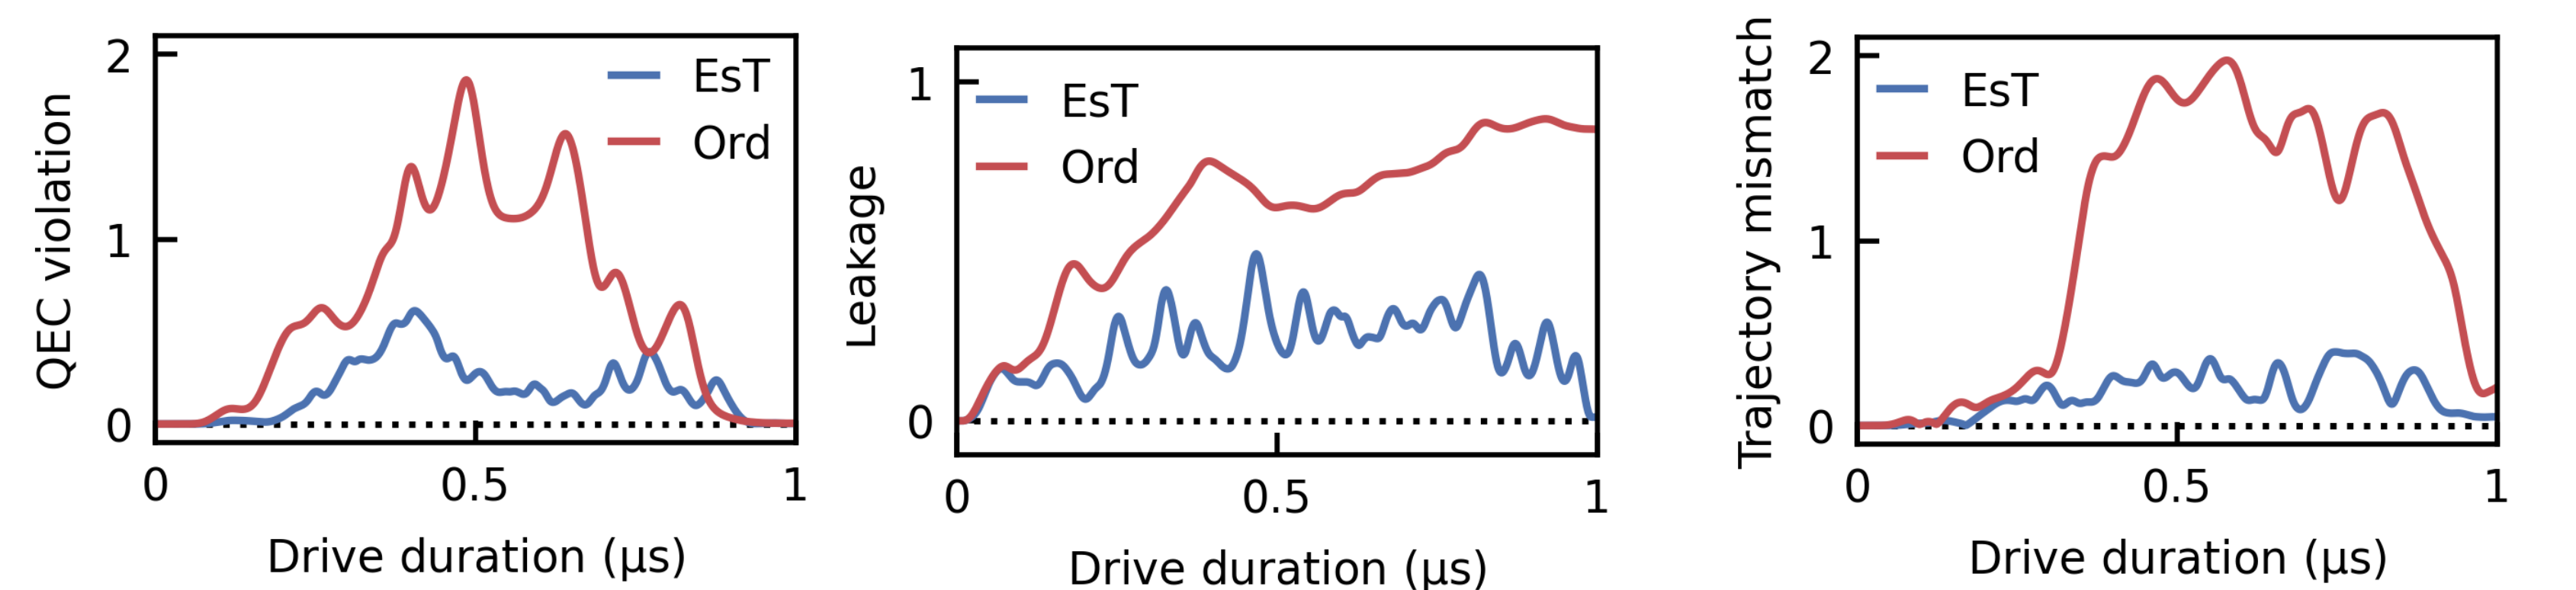
\includegraphics[width=0.78\textwidth]{img/paper_fig1def.png} \\[0.2em]
    \rotatebox{90}{\hspace{2.2em}\scriptsize\textbf{Ours}, Fig.~2a} &
      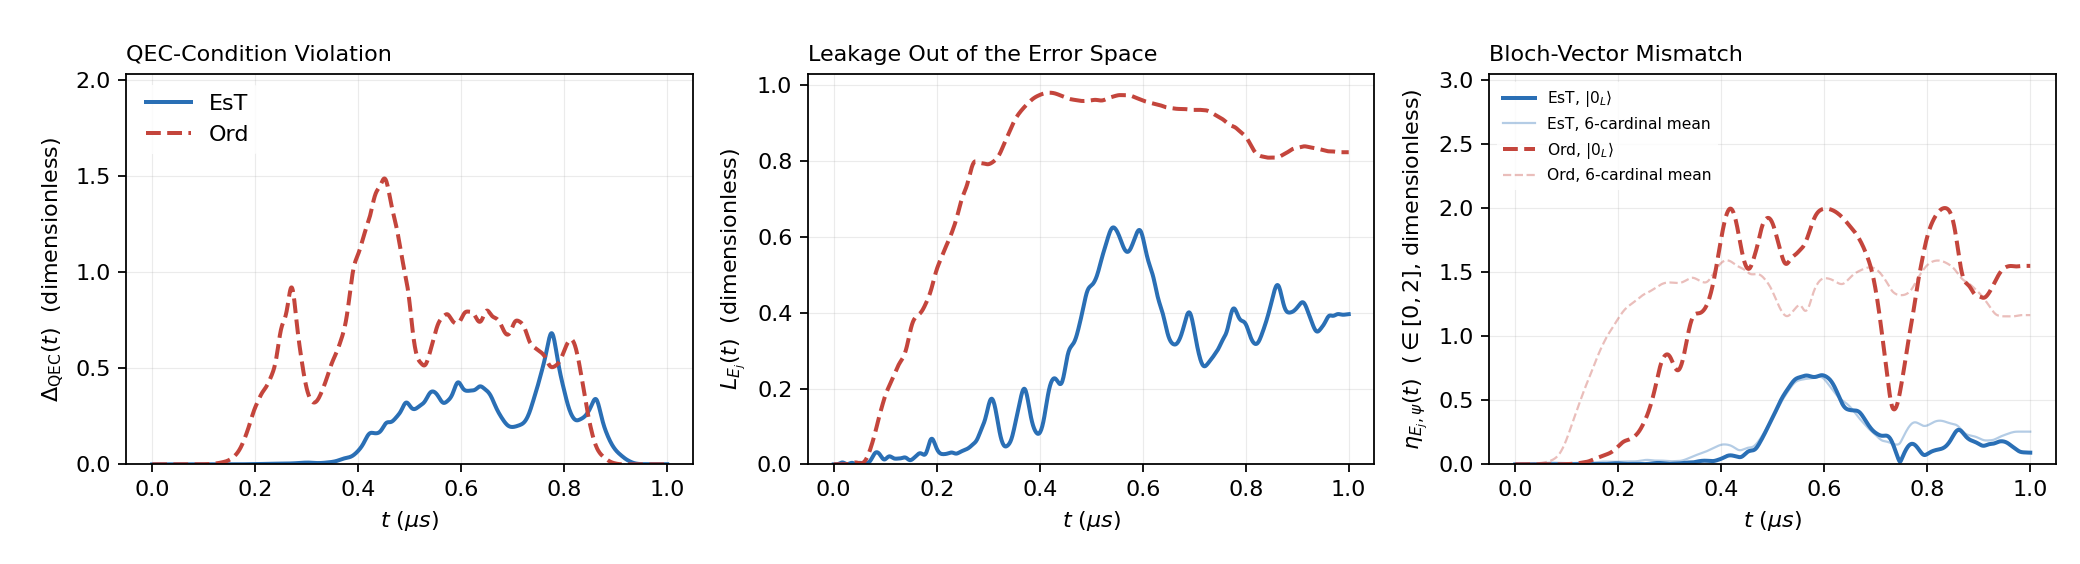
\includegraphics[width=0.93\textwidth]{img/ours_fig2a.png}
  \end{tabular}

  \smallskip
  {\color{tagmid}\scriptsize Left to right: $\dqec$, $L$, $\eta$ for $\ket{0_L}$ (ours also
  shows the six-cardinal mean, faint). $X$ gate, $1\,\mu$s, lossless simulation, linear axes.
  EsT blue, Ord red.}
  \note{
    \begin{ntitem}
      \item Same three metrics, same gate, same duration, same linear axes. Top row is the
            paper's Fig.~1d--f, cut from the PDF; bottom row is our own Figure~2a from
            \texttt{est\_experiments.ipynb}, recomputed from our trained pulses.
      \item Read it column by column. Left, QEC violation: both start and end near zero,
            because both pulses bring the code words back into the code at $t=T$; Ord peaks
            mid-pulse in both, EsT stays lower through the middle.
      \item Middle, leakage: Ord climbs towards 0.8--1 in both. The EsT curves are at a
            similar level mid-pulse. The visible difference is the very end: the paper's EsT
            drops to zero at $t=T$, ours stays near 0.4.
      \item Right, trajectory mismatch for $\ket{0_L}$: Ord reaches the maximum of 2 in both,
            EsT stays well below. At the very end the paper's Ord falls back to about 0.2;
            ours stays near 1.5.
      \item Our legend says ``Bloch-vector mismatch'' and the paper says ``trajectory
            mismatch''; it is the same Eq.~8.
      \item The next slide puts numbers on this.
    \end{ntitem}}
\end{frame}

% ------------------------------------------------------------------ results: numbers
\begin{frame}{What agrees, and what does not}
  \slidelabel{cmpnum}%
  \begin{center}
  \small
  \renewcommand{\arraystretch}{1.2}
  \begin{tabular}{@{}l l l@{}}
    \textbf{$X$ gate, EsT / Ord} & \textbf{Paper} & \textbf{Ours} \\
    \hline
    $L$, time-averaged          & 0.22 / 0.61 \;{\color{tagmid}\scriptsize digitised}
                                & 0.258 / 0.740 \\
    Ord : EsT on $L$            & 2.74            & 2.87 \\
    $L(T)$, end of gate         & 0.013 / 0.862   & \textbf{0.396} / 0.824 \\
    $\dqec$, peak               & $\approx$0.6 / $\approx$1.9 & 0.68 / 1.49 \\
    $\eta(\ket{0_L})$ at $t=T$  & $\approx$0.05 / $\approx$0.2 & 0.09 / \textbf{1.55} \\
    \hline
  \end{tabular}
  \end{center}
  {\color{tagmid}\scriptsize $\approx$: read by eye from the paper's figure.}

  \medskip
  \begin{columns}[T, onlytextwidth]
    \begin{column}{0.48\textwidth}
      \textbf{\color{codegreen}Agrees}
      \begin{itemize}
        \item EsT below Ord through mid-pulse, on all three.
        \item Leakage level and Ord:EsT ratio within about 20\%.
      \end{itemize}
    \end{column}
    \begin{column}{0.48\textwidth}
      \textbf{\color{ordred}Differs}
      \begin{itemize}
        \item The end of the gate: their EsT finishes transparent, ours still leaks.
        \item Our late $\dqec$ peak (0.78~$\mu$s).
      \end{itemize}
    \end{column}
  \end{columns}
  \note{
    \begin{ntitem}
      \item Where the numbers come from. Paper leakage: digitised from Fig.~1e in the
            notebook (400 and 600 dpi agree to 0.002). Paper endpoint values and peaks: read off
            the figure by eye, good to about 0.05--0.1. Ours: computed from the trained pulses
            with the eigh propagator.
      \item The good news first. Time-averaged leakage is 0.258 against their 0.22 for EsT,
            and the Ord-to-EsT ratio is 2.87 against 2.74. Same metric, same gate, same
            ballpark: the replication is in the right place on average.
      \item Peaks: our Ord QEC violation tops out at 1.5 against their 1.9; EsT is about the
            same height, 0.68 vs 0.6, but ours peaks late, at 0.78~$\mu$s, where theirs peaks at
            0.40~$\mu$s.
      \item The real difference is the endpoint, in bold. Their EsT gate finishes with leakage
            0.013, essentially transparent. Ours finishes at 0.396. Their Ord pulse also
            returns to a small trajectory mismatch at $t=T$ (about 0.2); ours ends at 1.55.
      \item Why the endpoint matters: QEC runs at $t=T$. A gate that is transparent on average
            but leaks at the end hands the recovery an error state in the wrong place.
    \end{ntitem}}
\end{frame}

% ------------------------------------------------------------------ results: why the endpoint differs
\begin{frame}{Why the endpoint differs, and caveats}
  \slidelabel{cmpwhy}%
  \begin{block}{The end-of-gate leak}
    \begin{itemize}
      \item \textbf{Not the printed cost form.} Retraining with the paper's own $C_2$ and $C_3$
            leaves $L(T)$ at about 0.4.
      \item \textbf{A terminal error-space term fixes it.} Adding error-space fidelity at
            $t=T$: $L(T)$ $0.40 \to 0.005$ at $F_1 = 0.9995$ (one seed).
      \item \textbf{Hypothesis:} the paper's EsT gate ``optimizes for fidelity of operation in
            both code and error space'' (App.~C), but no such term is printed.
    \end{itemize}
  \end{block}

  \begin{block}{Caveats}
    One seed per variant. Fock levels are not matched (EsT 9, Ord 8; the paper matches
    them). Paper values are digitised or read by eye.
  \end{block}
  \note{
    \begin{ntitem}
      \item We tested the obvious explanation first. Our $C_2$ and $C_3$ differ from the printed
            equations, so we retrained $X$ with the printed forms at the same weights, at two
            seeds. $L(T)$ came out 0.40 and 0.39 against 0.38 and 0.40 with ours: no change
            (notebook Appendix~A).
      \item Then the constructive test: add a cost on the error-space fidelity at the final
            time. On a comparable run (seed 6, baseline $L(T) = 0.398$) it brings $L(T)$ to
            0.005, with gate fidelity 0.9995 and the time-averaged transparency unchanged. One
            seed (\texttt{est\_optimization.ipynb}, section 1).
      \item So the leak is a property of the objective, not of the device. The paper's text
            says the EsT gate optimises fidelity in both code and error space, but its printed
            cost (Eqs.~C1--C8) has no error-space fidelity term. Our guess is that their code
            has one. Present this as a hypothesis we cannot check without their code.
      \item Caveats, plainly. Each comparison is one EsT and one Ord pulse. The paper compares
            pulses matched in maximum active Fock level; ours are 9 and 8, so our ratios are
            provisional. And their numbers come from digitising or reading a figure.
    \end{ntitem}}
\end{frame}

% ------------------------------------------------------------------ limitations
\section{Limits}

\begin{frame}{What this approach does not cover}
  \begin{itemize}
    \item \textbf{Only cavity photon loss is made transparent.} Transmon decay and dephasing
          during the gate are not. With $T_{2,R}^{q} = 30\ \mu$s against a $1\ \mu$s gate,
          they are comparable to cavity loss ($\bar n\,T/T_1 \approx 1$--$2\%$).
    \item \textbf{Single loss only.} Two photons lost in one gate are not covered.
    \item \textbf{The optimisation is lossless.} It never trades transparency against
          decoherence: nothing stops a pulse buying transparency with extra time in $\ket{e}$.
    \item \textbf{Model vs.\ hardware.} Line distortion and mixer imbalance are not modelled,
          and the $\ket{f}$ shift is taken as $2\chi$ (from $\chi\,\ad\aop\,\qd\qop$).
    \item \textbf{Exact transparency is not reached}, by design
          (slide~\slideref{obstruction}).
  \end{itemize}
  \note{
    \begin{ntitem}
      \item Say these before anyone asks; the first one is the question a cQED PI asks first.
      \item Transmon errors: the whole framework is about the cavity jump $\aop$. A transmon
            $T_1$ event or dephasing mid-gate is not transparent. The numbers: a 1~$\mu$s gate
            against $T_2$ (Ramsey) of 30~$\mu$s and $T_1$ of 70~$\mu$s, versus cavity loss
            probability $\bar n T/T_1 \approx 2/180$ to $4/180$. Same order. The paper notes its
            approach is compatible with detectable-ancilla schemes; that is future work.
      \item Single loss: the code corrects one photon loss. Two in one gate is second order and
            outside the framework.
      \item Lossless optimisation: decoherence enters only when a pulse is scored afterwards.
            The optimiser has no reason to keep the transmon in $\ket{g}$ when it does not
            need it.
      \item Model: our simulation drives the ideal Hamiltonian. The real pulse passes through
            mixers and lines that distort it. And $\chi\,\ad\aop\,\qd\qop$ makes the $\ket{f}$
            level shift by exactly $2\chi$ per photon, which a real transmon need not do.
      \item Last: the floor in the metrics is expected, not a bug.
    \end{ntitem}}
\end{frame}

\section{Summary}

% ------------------------------------------------------------------ summary
\begin{frame}{Summary}
  \small
  \begin{enumerate}
    \item \textbf{QEC while idling}: Knill--Laflamme, $\PC E_a^{\dagger}E_b\PC \propto \PC$.
          The kitten code meets it, and parity is the syndrome.
    \item \textbf{Gates break it}: a loss at a random time gives a $t$-dependent endpoint.
          Error transparency asks the jump to commute through the gate.
    \item \textbf{Exact ET is not expected} with linear drives: Kerr and $\chi'$ leave an
          uncorrectable $\ad\aop^2$. Hence ``semi''.
    \item \textbf{Moving subspaces} $\Cs(t)$, $\Es_j(t)$: three conditions, and three metrics
          that measure them along the whole pulse.
    \item \textbf{GRAPE} shapes a staircase of real I/Q controls on a lossless model of the
          device.
    \item \textbf{The cost}: $C_1$ fidelity at the end, $C_2$ transparency at every step, $C_3$
          to spread the dynamics over the gate, in two stages. Ord is $C_1$ alone.
    \item \textbf{Constraints}: 50 MHz bandwidth, 4 MHz amplitude, 48 ns ramps, 1 ns steps.
  \end{enumerate}

  \vfill
  \centering
  {\color{estblue}\textbf{The trade:} give up exact transparency, keep the standard linear
  cQED toolkit, and optimise for as much transparency as it allows.}
  \note{
    \begin{ntitem}
      \item Walk the chain once, fast --- one sentence per item. The audience should hear it
            as a single argument: what is wrong, why it cannot be fully fixed, how to measure
            it, and how to optimise against it.
      \item Items 1--4 are the theory; items 5--7 are the optimisation. The bridge between
            them: the metrics measure transparency, but the optimiser uses a cheaper overlap,
            $C_2$, that pushes in the same direction.
      \item Land on the trade. The authors are not claiming exact transparency; they are
            claiming a favourable exchange rate.
      \item The number that makes the trade look good, as a teaser for the results talk: a
            five-fold reduction in logical infidelity conditioned on a photon loss during the
            gate, and a seventeen-fold reduction in per-gate error-space infidelity for $X$.
      \item Results are a separate talk: the metrics on real pulses, EsT versus Ord versus LE,
            and the experimental Wigner tomography.
      \item Invite questions on the two deviations we made from the printed equations ($C_2$
            and $C_3$ normalisation) --- they are the most likely thing a careful reader asks.
    \end{ntitem}}
\end{frame}

\section{Our replication}

% ------------------------------------------------------------------ replication status
\begin{frame}{Our replication: status and open questions}
  \slidelabel{replication}%
  \begin{columns}[T, onlytextwidth]
    \begin{column}{0.53\textwidth}
      \textbf{Done} {\color{tagmid}\small(simulation only)}
      \begin{itemize}
        \item Independent model and cost, with two gradient codes (autodiff and hand-derived)
              that agree.
        \item $X$, $H$, $T$ trained, EsT and Ord, with two documented changes to the printed
              cost ($C_2$, $C_3$).
        \item On $X$ and $H$, EsT lowers leakage and trajectory mismatch about 3--7$\times$
              against Ord (one seed; slide~\slideref{cmpnum}).
        \item Extra costs tried ($\Delta\bar n$, end-of-gate error-space fidelity,
              smoothness): each moves its own target; none is a free win.
      \end{itemize}
    \end{column}
    \begin{column}{0.43\textwidth}
      \textbf{Open}
      \begin{itemize}
        \item Seed-to-seed spread of the EsT--Ord gap.
        \item End-of-gate leakage: $L(T) \approx 0.4$ on $X$, against the paper's 0.013
              (slide~\slideref{cmpwhy}).
        \item Transmon errors are outside the model.
        \item A Fock-matched, multi-seed comparison with the paper.
      \end{itemize}
    \end{column}
  \end{columns}
  \note{
    \begin{ntitem}
      \item Keep this to what we have shown. Everything here is simulation; we have not run
            hardware.
      \item Two gradient codes: a JAX autodiff path and a numpy path with a hand-derived
            gradient. They are checked against each other and against finite differences.
      \item The two cost changes are the $\mathcal{N}^2$ in $C_2$ and the unit-free $C_3$,
            both explained on their slides.
      \item The 3--7 times is time-averaged leakage and Bloch mismatch, EsT against Ord. $X$:
            leakage 2.9 times, mismatch 6.6 times on $\ket{0_L}$. $H$: 4.5 and 5.2 times. Single
            seed for these headline pairs.
      \item Extra costs: the mean-photon-number penalty halves $\dqec$ but hurts leakage; an
            end-of-gate error-space fidelity term cuts $L(T)$ but can stall some seeds; a
            smoothness term raised the mismatch. The metrics trade against each other.
      \item Open: the end-of-gate leakage of about 0.4, against the paper's 0.013. The results
            slides show a terminal error-space term removes it; whether that is what the paper
            did is the question. And we need more seeds before quoting any EsT--Ord ratio as a result.
    \end{ntitem}}
\end{frame}

\appendix
\renewcommand{\framenumprefix}{B}
\section{Backup}

% ------------------------------------------------------------------ why KL suffices (1/2)
\begin{frame}{Why that condition is enough (1/2): untangle the errors}
  \slidelabel{klproof}%
  {\color{tagmid}\small Shorthand on these backup slides: $P \equiv \PC$.}

  \smallskip
  \begin{enumerate}
    \item $\alpha$ is Hermitian, so a unitary $u$ diagonalises it:
      \[
        \alpha = u\,d\,u^{\dagger}, \qquad d = \mathrm{diag}(d_k), \quad d_k \ge 0 .
      \]
    \item Recombine the Kraus operators with it (same channel, slide~\slideref{setup}):
      \(F_k = \sum_a u_{ak}\,E_a\).
      \medskip
    \item The error-correction condition becomes
      \[
        P\,F_k^{\dagger}F_l\,P
        = (u^{\dagger}\alpha\,u)_{kl}\,P
        = d_k\,\delta_{kl}\,P .
      \]
  \end{enumerate}

  \begin{block}{Only the diagonal survives}
    Different errors $F_k \neq F_l$ no longer overlap on the code, and error $k$ occurs
    with probability $d_k$ whichever codeword it hits.
  \end{block}
  \note{
    \begin{ntitem}
      \item Use the non-uniqueness from two slides ago. That freedom is the whole trick.
      \item Step 1: $\alpha$ is Hermitian (in fact a Gram matrix, so positive
            semidefinite), so it has a unitary eigenbasis and real, non-negative
            eigenvalues $d_k$.
      \item Step 2: rotate the Kraus set by that same unitary. Same channel, new labels.
      \item Step 3: substitute.
            $P F_k^{\dagger}F_l P = \sum_{a,b} \bar u_{ak}\,\alpha_{ab}\,u_{bl}\,P$,
            and that sum is just $(u^{\dagger}\alpha u)_{kl} = d_k\delta_{kl}$. Only the
            diagonal is left, hence the $\delta_{kl}$.
      \item What the $\delta_{kl}$ buys: the original $E_a$ could overlap on the code, so
            you could not cleanly tell them apart. The new $F_k$ cannot.
      \item What the $d_k$ means: $\|F_k\ket{\psi}\|^2 = d_k$ for every code state, so
            learning ``$k$ happened'' reveals nothing about the logical state.
      \item If some $d_k = 0$, that $F_k$ annihilates the code: it never happens on code
            states, so drop it.
    \end{ntitem}}
\end{frame}

% ------------------------------------------------------------------ why KL suffices (2/2)
\begin{frame}{Why that condition is enough (2/2): undistorted copies}
  Normalise each error on the code:
  \[
    V_k \equiv \frac{1}{\sqrt{d_k}}\,F_k P .
  \]

  \medskip
  Each $V_k$ is a \textbf{partial isometry}: it maps $\Cs$ onto an image
  $\Cs_k = V_k\Cs$ without distorting it, and
  \[
    V_k^{\dagger}V_k = P, \qquad V_k^{\dagger}V_l = 0 \;\; (k\neq l).
  \]

  \medskip
  So the errors scatter the code into \textbf{disjoint, orthogonal, undistorted copies}
  of itself.

  \medskip

  \medskip
  {\color{tagmid}\small Correcting a discrete set also corrects its entire linear span, so
  discrete errors suffice.}
  \note{
    \begin{ntitem}
      \item Both identities are the previous slide's equation divided by $d_k$: set $k=l$
            for the first, $k\neq l$ for the second.
      \item Partial isometry: $V_k$ preserves every inner product inside $\Cs$ and kills
            everything outside it. So on the code, $F_k$ is $\sqrt{d_k}$ times a rigid
            move. The image $\Cs_k$ is an undistorted copy of $\Cs$, and different $k$ give
            orthogonal copies.
      \item Set up the next slide: that geometry \emph{is} what makes recovery possible.
            Orthogonal copies can be told apart by a measurement; undistorted copies can be
            rotated back.
      \item Closing remark on linearity: if $R$ corrects $\{E_a\}$ it corrects any
            $F_r = \sum_a M_{ra}E_a$, because $R_kF_rP \propto P$ still. That is why we may
            restrict attention to a discrete error set.
    \end{ntitem}}
\end{frame}


% ------------------------------------------------------------------ recovery
\begin{frame}{Recovery: find the copy, rotate it back}
  \slidelabel{klrecovery}%
  After the noise, the code sits on copy $k$ with probability $d_k$:
  \(
    \varepsilon(\rho) = \sum_k d_k\, V_k\,\rho\,V_k^{\dagger} .
  \)

  \medskip
  \begin{enumerate}
    \item \textbf{Error-space projector} onto $\Cs_k = V_k\Cs$:
      \[
        P_k = V_kV_k^{\dagger}, \qquad P_kP_l = \delta_{kl}\,P_k .
      \]
    \item \textbf{Measure} $\{P_k\}$. Outcome $k$ and the state it leaves:
      \[
        p_k = \Tr\!\big[P_k\,\varepsilon(\rho)\big] = d_k ,
        \qquad \varepsilon(\rho) \;\to\; V_k\,\rho\,V_k^{\dagger} .
      \]
    \item \textbf{Rotate back} with $V_k^{\dagger}$:
      \[
        V_k^{\dagger}\big(V_k\,\rho\,V_k^{\dagger}\big)V_k = P\rho P = \rho .
      \]
  \end{enumerate}

  \medskip
  {\color{tagmid}\small $p_k = d_k$ for every $\rho$: the syndrome reveals the error, never the
  logical state.}
  \note{
    \begin{ntitem}
      \item The previous slide built the geometry. This one runs the protocol on it.
      \item Starting point: $F_lP = \sqrt{d_l}\,V_l$, so the noisy state is a mixture. With
            probability $d_l$ the code was moved rigidly onto copy $l$; we do not yet know
            which.
      \item Step 1: $P_k$ is a projector because $V_k^{\dagger}V_k = P$ and $V_kP = V_k$,
            so $P_k^2 = V_kPV_k^{\dagger} = P_k$. Different copies are orthogonal because
            $V_k^{\dagger}V_l = 0$. Add $\id - \sum_k P_k$ to complete the measurement; that
            outcome never fires.
      \item Step 2: on a single branch, $P_kF_l\ket{\psi} = \delta_{kl}F_l\ket{\psi}$. So
            the outcome is certain and the state is not disturbed --- it was already an
            eigenstate of the projector.
      \item The key point: $p_k = d_k$ does not depend on $\rho$. The measurement asks only
            a question whose answer is the same for every code state, so it learns the
            error and nothing about the logical information. That is the
            ``$\alpha_{ab}$ independent of $i$'' half of Knill--Laflamme, seen as a
            property of the measurement.
      \item Step 3: $V_k^{\dagger}$ is not unitary on the whole space. In the lab you apply
            any unitary that agrees with $V_k^{\dagger}$ on $\Cs_k$; one always exists
            because $\Cs_k$ and $\Cs$ have the same dimension.
      \item Order matters: measure first, then pick $V_k^{\dagger}$ (feedback). Averaged
            over outcomes, $\sum_k V_k^{\dagger}\varepsilon(\rho)V_k = \sum_k d_k\,\rho = \rho$,
            since completeness of the Kraus set gives $\sum_k d_k = 1$.
      \item Kitten preview: the copies are the even and odd parity sectors, so the
            syndrome is a parity measurement.
      \item Key sentence: the parity check we use in the lab is not an extra ingredient ---
            it is the projective measurement that Knill--Laflamme forces into existence.
    \end{ntitem}}
\end{frame}
